\chapter{Supplementary Discussions} \label{chap:supdiscussions}

\section{Machine Learning Overview towards Atomistic Materials Science} \label{sipfenn:appedix1}
The class of deep learning methods has been remarkably successful in recent years in applications ranging from computer vision to natural language processing and simulations of quantum systems \cite{lecun2015deep,silver2016mastering,devlin2018bert,carleo2017solving}. Although deep neural networks have existed for a long time \cite{rosenblatt1958perceptron}, and had been successfully applied to computer vision tasks \cite{lecun1995comparison,lecun1990handwritten,lecun1998gradient}, a major breakthrough was the \texttt{AlexNet} network \cite{krizhevsky2012imagenet}, which dramatically improved the accuracy achievable on large-scale image classification. Following this success, deep neural networks have been very intensively studied and applied to a variety of problems \cite{lecun2015deep,silver2016mastering,devlin2018bert}. Deep neural networks are particularly effective when applied to regression problems, where one is learning a functional relationship between a feature and a prediction. For many problems, deep neural networks are able to achieve significantly better performance than competing machine learning methods, due to their ability to learn more complex relationships. With materials science being a field where many complex dependencies are intertwined, it is to be expected that this superior pattern recognition can carry over to the improvement in the prediction of material properties.

\subsection{Regression Problem Formulation and Artificial Neural Networks}
\label{sipfenn:ssec:regressionformulation}

The general formulation of a regression problem in statistical machine learning is to find a function $f:X\rightarrow Y$ which minimizes the risk \cite{vapnik1999overview}, also known as loss or expected error.
\begin{equation}\label{sipfenn:true_risk_app}
    R(f) = \mathbb{E}_{x,y\sim \mathcal{P}} l(y,f(x)).
\end{equation}
Here $X$ denotes a space of input features, $Y$ denotes an output space, the expectation above is taken over an unknown distribution $\mathcal{P}$ on $X\times Y$ (representing the true relationship between inputs and outputs), and $l$ is a given loss function. The goal is to find a function $f$ which accurately predicts the (potentially random) output $y$ given an input $x$.

In the present work, $x\in X$ represents the input features (descriptor) characteristic of the material, and $y\in Y$ represents the formation energy. The distribution $\mathcal{P}$ represents the true material-property relationship between given descriptor $x$ and corresponding formation energy. This relation may not be as simple as mapping a given structure to an energy since different DFT methodologies may give different results, based on many variables, such as employed functionals. \cite{CharlesW.BauschlicherJr.1995AFunctionals, Alturk2017ComparisonMaterial} Consequently it is useful to describe this relationship via a probability distribution. Furthermore, the loss function considered in the present paper is the commonly used $\ell^1$ or absolute error (AE) loss function $l(y_1,y_2) = |y_1-y_2|$. %modified this since we are using l1, not l2 - Adam

In practice, the distribution $\mathcal{P}$ is not known. Indeed it is this relationship that one is trying to learn in the first place. Instead, what is available is data $\{(y_i,x_i)\}_{i=1}^n$, which is sampled from $\mathcal{P}$. From this one forms the empirical risk \cite{hastie2009elements,vapnik2013nature}
\begin{equation}\label{sipfenn:empirical_risk_app}
    L(f) = \frac{1}{n}\displaystyle\sum_{i=1}^n l(y_i, f(x_i)),
\end{equation}
and seeks a function $f$ which minimizes the empirical risk, also known as the training error.

In addition, one must specify the type of relationship that is expected to be found between the inputs $x_i\in X$ and the predictions $y_i\in Y$. This is done by restricting the function $f$ to a specific class. For instance, by restricting $f$ to be linear, which corresponds to looking for a linear relationship between $x_i$ and $y_i$, one obtains a linear regression. On the other hand, choosing $\mathcal{F}$ to be a reproducing kernel Hilbert space of functions on $X$ with the same loss $l$ one obtains the kernel ridge regression method. Thus in order to fit the model, the training error is minimized over a specific class of function $\mathcal{F}$, i.e. one solves the optimization problem
\begin{equation}\label{sipfenn:empirical_risk_min_eq}
    f^* = \arg\min_{f\in \mathcal{F}} L(f) = \arg\min_{f\in \mathcal{F}} \frac{1}{n}\displaystyle\sum_{i=1}^n l(y_i, f(x_i)).
\end{equation}

In this the class of functions $\mathcal{F}$ is chosen as the set of functions defined by a neural network architecture (schematic in Figure \ref{sipfenn:fig:nnschematic}), which leads to a deep learning method. A neural network architecture consists of a sequence of alternating linear functions and point-wise non-linear functions \cite{goodfellow2016deep}. In the figure \ref{sipfenn:fig:nnschematic} the nodes, or neurons, represent applications of a point-wise non-linear function, called an activation function, and the connections between nodes represent linear functions from the output of the nodes in one layer to the input of the next layer.

\begin{figure}[H]
    \centering
    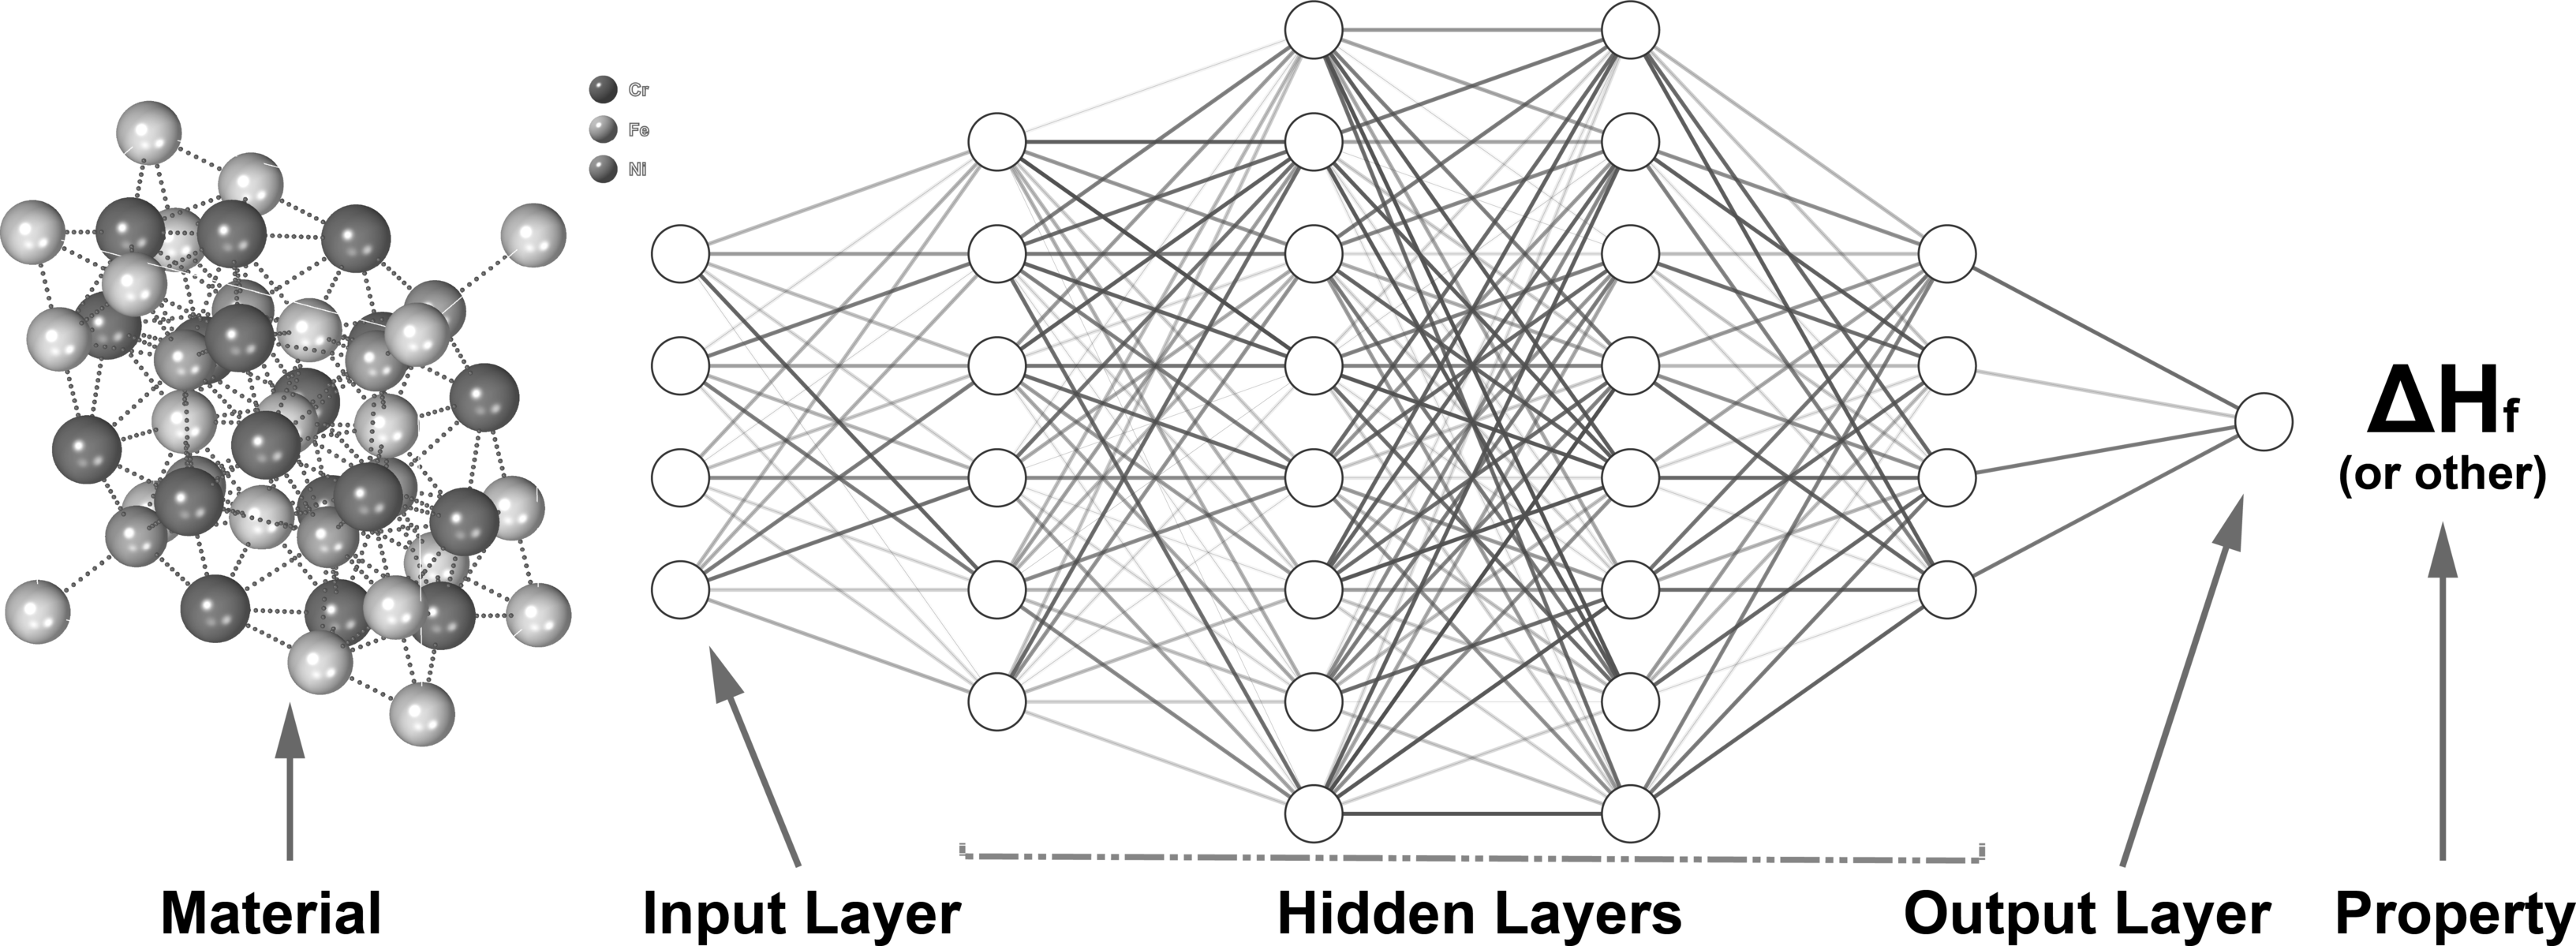
\includegraphics[width=0.85\textwidth]{sipfenn/NN_schematic.png}
    \caption{Simplified artificial neural network schematic}
    \label{sipfenn:fig:nnschematic}
\end{figure}

The class of functions represented by the neural network consists of the functions obtained by substituting different linear maps between each layer. Specifically, given weight matrices $W_1,...,W_n$ and biases $b_1,...,b_n$, which are parameters of the network, the corresponding neural network function is given by the composition

\begin{equation}
    f_{W_1,...,W_n,b_1,...,b_n}(x) = W_n\cdots\sigma(W_3\sigma(W_2\sigma(W_1x+b_1)+b_2)+b_3)\cdots + b_n
\end{equation}

where $\sigma$, called the activation function, is applied pointwise to each entry of the vector input (previous layer output). The neural network architecture is determined by the type, dimensionality, activation function $\sigma$, and arrangement of intermediate layers. This can potentially introduce some additional restrictions on the linear maps $W_i$, see for instance convolutional neural networks, where the linear maps $W_i$ are restricted to be convolutions with small kernels \cite{krizhevsky2012imagenet,lecun1995comparison,lecun1998gradient}.


Once the neural network architecture has been set, one must fit the values of the parameters $W_1,...,W_n$ and $b_1,...,b_n$ by optimizing the training loss $L$,

\begin{equation}
    \arg\min_{W_1,...,W_n,b_1,...,b_n} L(f_{W_1,...,W_n,b_1,...,b_n}).
\end{equation}

This optimization problem is typically solved using stochastic gradient descent \cite{lecun1998gradient}, or a more robust method such as ADAM \cite{kingma2014adam}, which was used in the present work. To solve the problem faster and to mitigate overfitting, which is discussed in the next sections, these methods form an estimate of the loss function gradient by considering a small subset of the data, called a batch. Each training step is done over all of the data in the batch, so parameters ($w$ and $b$) are updated based on many data points, rather than a single one. Most of the models created in the present work used a batch size of 2,048 data points.

This methodology has been successfully applied to a variety of practical machine learning problems \cite{krizhevsky2012imagenet,goodfellow2013multi,dahl2011context}. Specifically relevant to the present work, neural networks have been applied to problems in computational materials science \cite{Huang2019Machine-learningAlloys,Feng2019UsingDefects}. For example, in \cite{Huang2019Machine-learningAlloys} neural networks are used to classify the phases of high-entropy alloys. For this application, their neural network models compare favorably to other machine learning algorithms such as $k$-nearest neighbor (KNN) and support vector machines (SVM). Furthermore, in \cite{Feng2019UsingDefects} it is shown that even when training on small datasets which are typical of certain materials science problems, specifically in the prediction of solidification defects from optical microscopy data, deep neural networks can achieve better performance than other machine learning models. This is enabled by using a stacked auto-encoder (shallow neural network) to pre-train the deep neural network, whose weights are then fine-tuned on the small dataset. the present work complements these studies by applying deep neural networks to the prediction of thermodynamic quantities from atomic structure descriptors.

\subsection{Overfitting and its Mitigation}
\label{sipfenn:ssec:overfitting}

\begin{figure}[h]
    \centering
    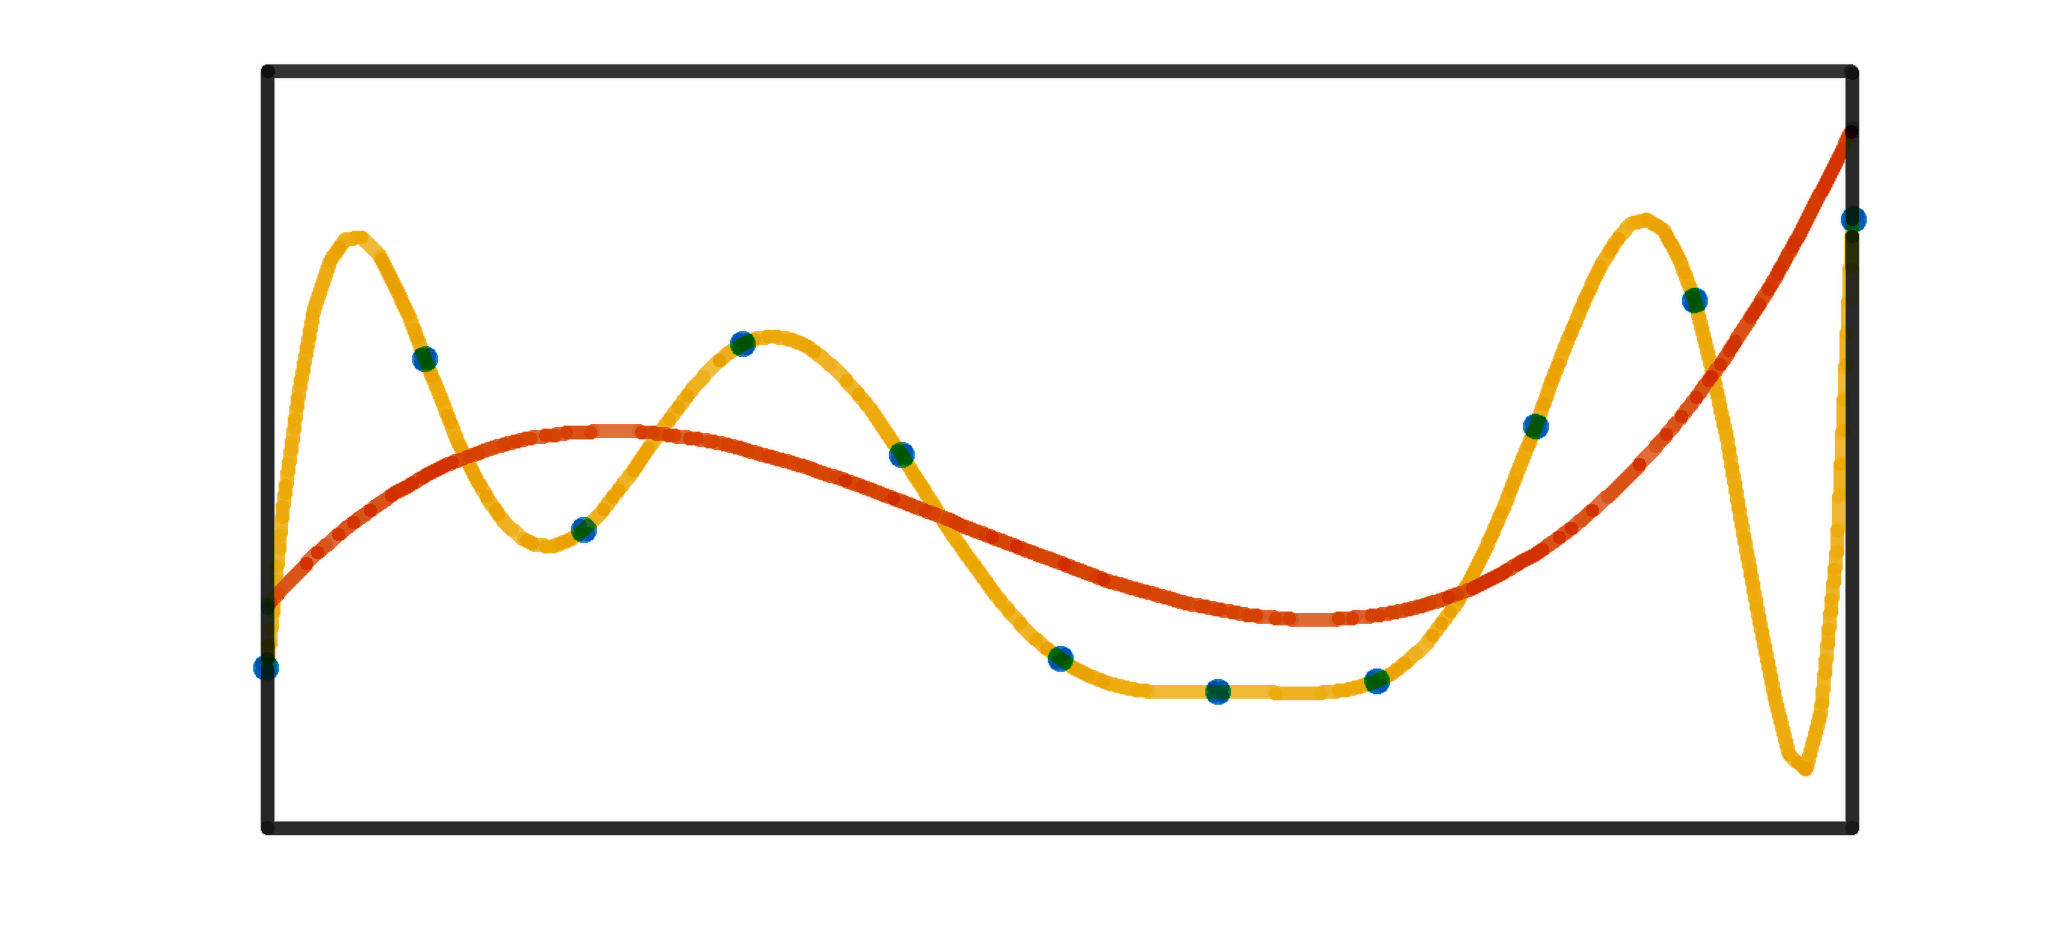
\includegraphics[width=0.5\textwidth]{sipfenn/overfitting.png}
    \caption{A schematic of overfitting. The overfit model (yellow) is too complex and memorizes the training data. This results in very low training error, but also very poor performance when predicting hidden data (test error) that follows the underlying phenomena (red).}
    \label{sipfenn:fig:overfitting}
\end{figure}

A major problem in statistical learning is avoiding overfitting \cite{hastie2009elements}, which, in simple terms, signifies that the model memorizes the training data instead of learning the true  relationship between descriptors $x$ and predictions $y$, as depicted in Figure~\ref{sipfenn:fig:overfitting}. This occurs when the class of functions $\mathcal{F}$ is too large, and at the optimal function $f^*$ in \eqref{sipfenn:empirical_risk_min_eq} the empirical \eqref{sipfenn:empirical_risk_app} and true risk \eqref{sipfenn:true_risk} diverge sharply. This results in very low training error, but poor performance on data that was not presented to the network.

Overfitting is typically detected by separating the training data into two sets, the data used in \eqref{sipfenn:empirical_risk_min_eq} to learn the function $f^*$, called the training data, and a separate set of data used to evaluate the performance of $f^*$, called the validation set. Consequently, in addition to the training loss in \eqref{sipfenn:empirical_risk_min_eq}, the validation error

\begin{equation}\label{sipfenn:validation_loss}
    L_{val} = \frac{1}{m}\displaystyle\sum_{i=1}^m l(\tilde{y}_i, f(\tilde{x}_i)),
\end{equation}

where $(\tilde{y}_i,\tilde{x}_i)$ for $i=1,...,m$ is the validation set, which was not presented to the network when adjusting its parameters, is used to detect overfitting. 
%%
The fraction of the data set aside for validation set should be large enough to be representative of the whole dataset to provide statistically significant conclusions, yet small enough so that knowledge loss in the process is minimized. In the present work, a randomly selected 15\% of every dataset has been used as validation sets for all training. This corresponded to 65,300 data points in the case of the OQDM dataset described in \ref{sipfenn:sssec:Data}.
%%

\begin{figure}{H}
    \centering
    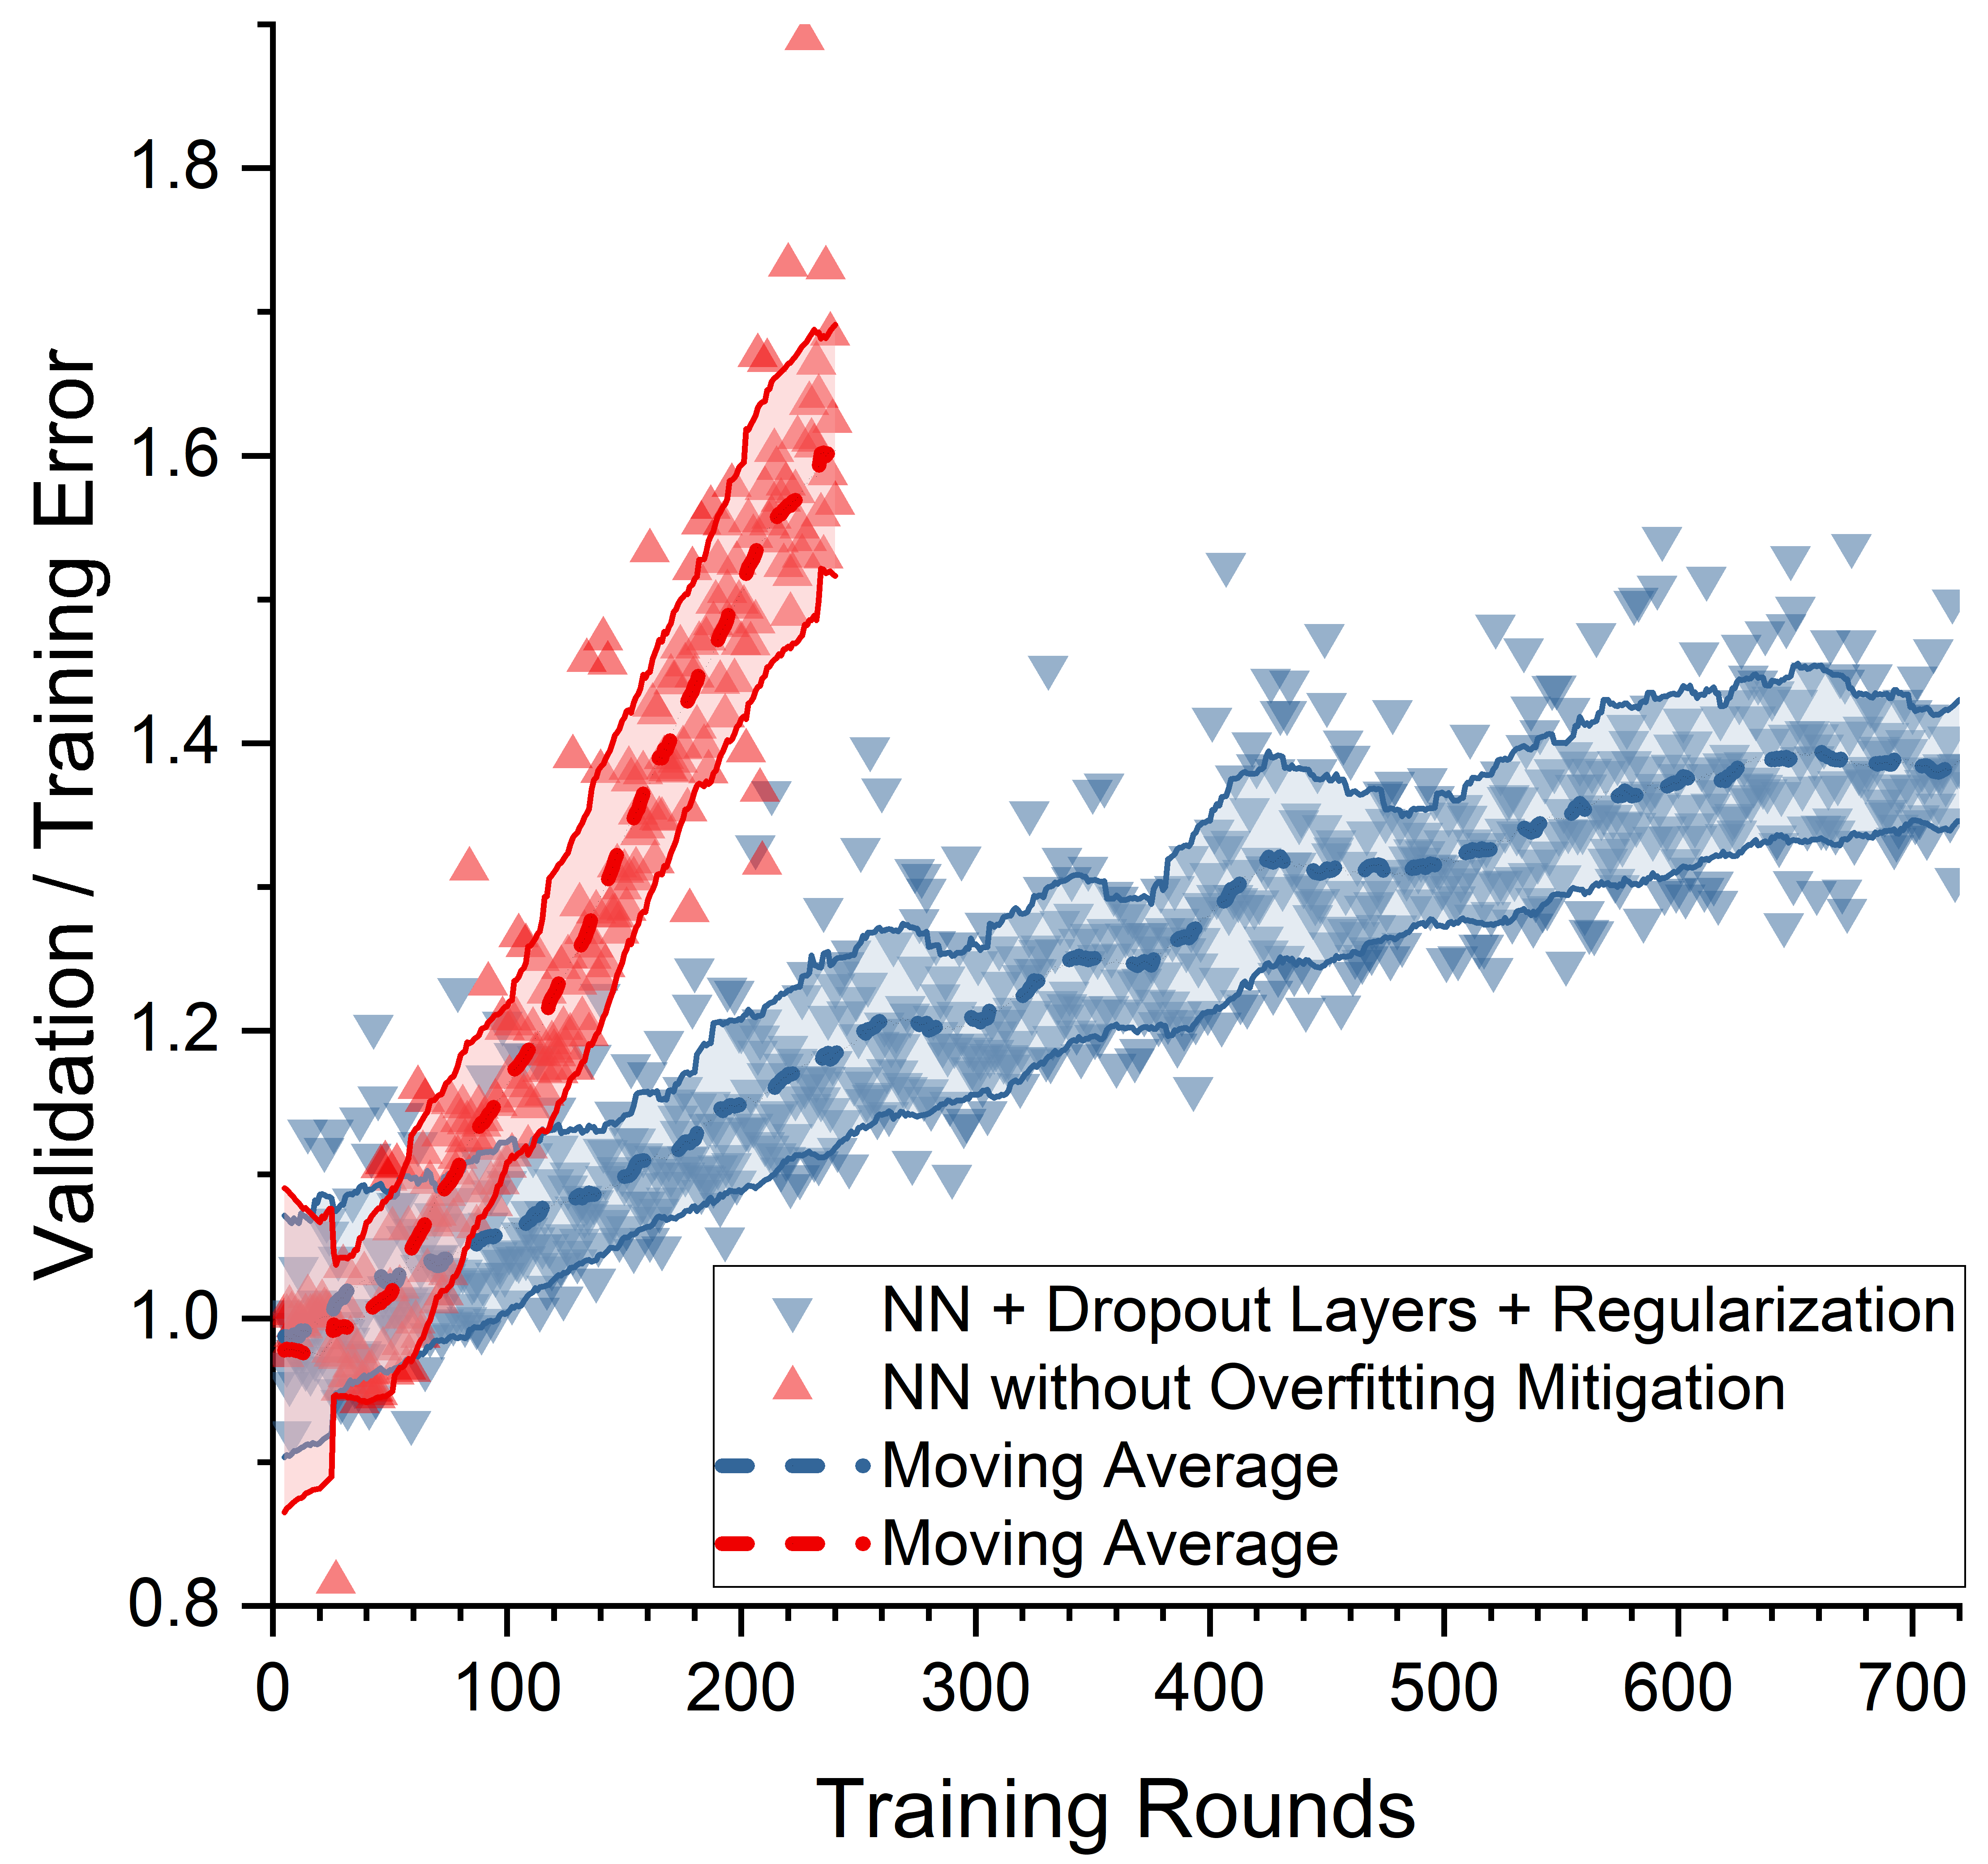
\includegraphics[width=0.65\textwidth]{sipfenn/validationtotraining_generalized.png}
    \caption{Training Loss to Validation Loss in a model that does without (NN9) and with overfitting mitigation (NN20), plotted versus training progress.}
    \label{sipfenn:fig:trainingvalidation}
\end{figure}

Typically, the validation loss will be greater than the training loss, as the validation set is not available for training. This is illustrated in Figure \ref{sipfenn:fig:trainingvalidation}, where the ratio between the validation loss \eqref{sipfenn:validation_loss} and test loss \eqref{sipfenn:empirical_risk_min_eq} during the course of two trainings of similar NN architectures on the same data with the same learning rate schedule has been plotted. This figure indicates that as the training proceeds, the gap between the training and validation errors widens and then increases. The size of this gap is an estimated measure of how much the model has overfitted to the data. In one of the models in this figure, extensive techniques to mitigate overfitting have been used, and for this model, the figure shows that the rate at which the model overfits to the data is much lower. At the same time both models exhibit similar performance on the test set.

There are numerous techniques used to prevent the issue of overfitting \cite{hastie2009elements,everitt2002cambridge}. These include utilization of a regularization term $\lambda R(\theta)$ added to the training error \eqref{sipfenn:empirical_risk_min_eq} to give the regularized empirical loss function

\begin{equation}
    f^* = \arg\min_{f\in \mathcal{F}} R_{emp}(f) + \lambda R(\theta).
\end{equation}

A standard regularizer typically added to the linear regression is the $\ell^2$-norm $R(\theta) = \|\theta\|_2^2$, which is often called Tikhonov regularization \cite{tikhonov1963solution} or ridge regression \cite{hoerl1970ridge}. The $\ell^2$-norm is also a popular regularizer in deep learning problems, where it is referred to as weight decay \cite{goodfellow2016deep}. In the context of the present work, it is implemented as a part of the training process, rather than network architecture, and causes rejection of some features in the descriptor that are not contributing to pattern recognition. Results of its implementation are shown throughout Section \ref{sipfenn:sssec:NetDesign}.

Another important method used to prevent overfitting in machine learning is the Dropout technique \cite{srivastava2014dropout}. The concept behind Dropout is to prevent neurons in the network from becoming overly dependent on the output from a specific neuron in the previous layer, often referred to as hard-wiring neuron paths. A Dropout layer, placed within a neural network, is implemented as a function operating during the training process and randomly discarding a specified fraction $p$ of previous layer outputs and multiplying the remaining values by $1/(1-p)$. This forces the pattern recognition ability to be dispersed across the network, as during evaluation of every training step, a random part of the network is acting as if it was not gone. Once the training is completed, all Dropout layers are deactivated and simply pass all information forward, so that the model returns to its deterministic character.

In the experiments performed in the present work, as later discussed in \ref{sipfenn:sssec:NetDesign}, both Dropout and weight decay were used to mitigate overfitting, with good effects shown in particular in Figure \ref{sipfenn:fig:trainingvalidation}.

Methods for avoiding overfitting typically come with one or more "hyperparameters" (i.e. parameters which control the training process) that can represent how much confidence is given to the training data versus prior knowledge. For instance, if a regularizer is used, the strength of the regularizer, $\lambda$, would be a hyperparameter. In the terms of the present work, it generally corresponds to how many features in the material descriptor can be considered non-essential to making predictions and therefore discarded systematically throughout the training. Furthermore, when using Dropout, the probability $p$ is also a hyperparameter. 

One typically trains the model on the training dataset using a number of different hyperparameters and then subsequently chooses the best set of them using the validation error. This allows the determination of hyperparameter values that are appropriate to the problem at hand. However, in order to ensure that the determined hyperparameter values are not overly specific to the validation set, the final accuracy of the model is evaluated on a test set that was not used at all during training \cite{hastie2009elements}.

\begin{figure}[H]
    \centering
    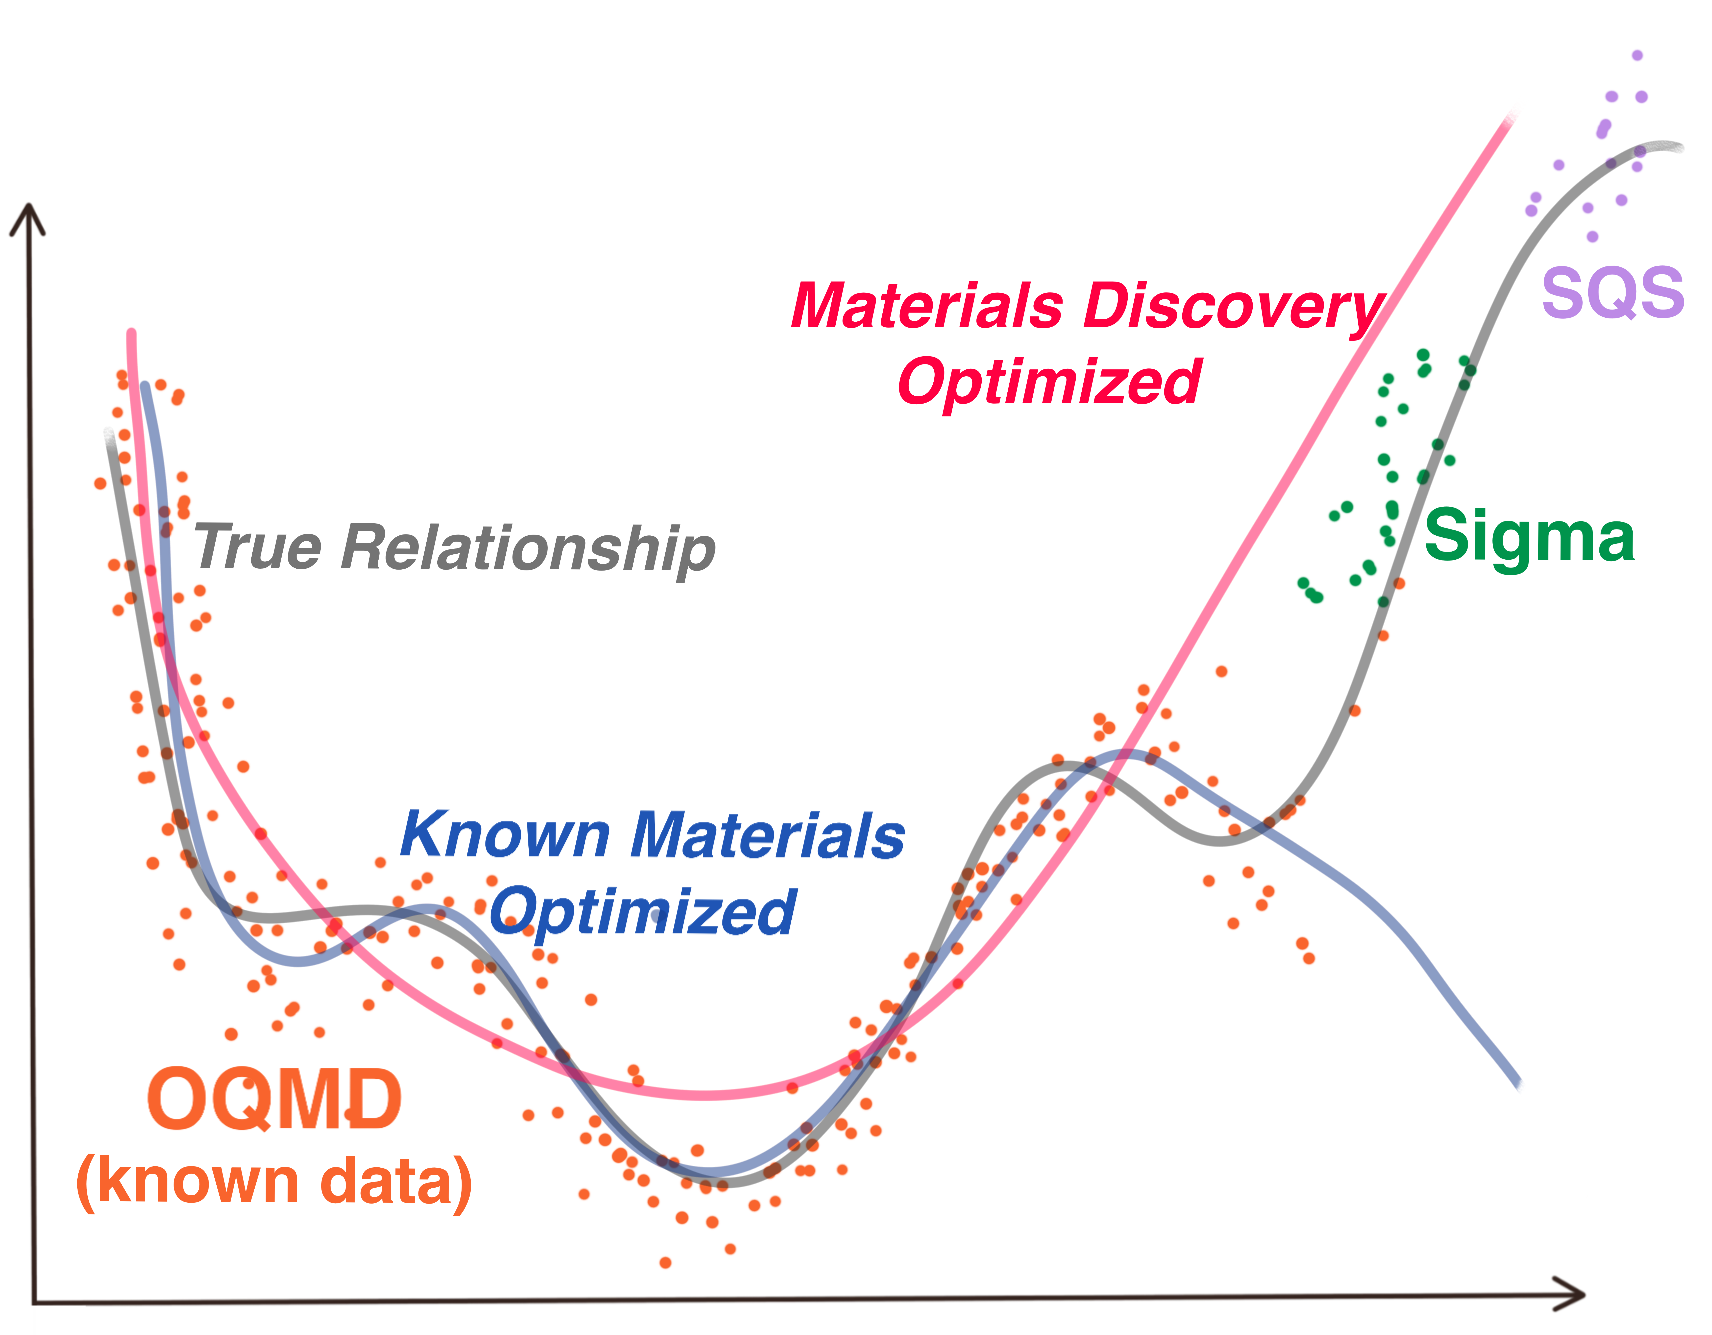
\includegraphics[width=0.7\textwidth]{sipfenn/Overfitting_discovery.png}
    \caption{A conceptual drawing depicting how overfitting mitigation effort can improve performance beyond regions with high known data density.}
    \label{sipfenn:fig:overfitting_newregions}
\end{figure}

An additional advantage of mitigating overfitting to known data can be increased performance during extrapolation, as depicted conceptually in Figure \ref{sipfenn:fig:overfitting_newregions}. This is thanks to reduced model complexity, which forces recognition of stronger and more broadly exhibited patterns rather than small deviations present in the training data, whether real or due to noise, that can significantly degrade the extrapolation capability of the ML model. It is important to recognize that cost of such model simplification is often reduced performance on previously unseen data that lays within the known region.


\subsection{Transfer Learning} \label{sipfenn:ssec:transferlearning}
Finally, one should consider the technique of transfer learning, which has been observed among deep learning models across a variety of domains \cite{tan2018survey,cirecsan2012transfer,chang2017unsupervised,george2018deep}. Transfer learning refers the to the ability of properly trained deep learning models to `transfer' their knowledge to related tasks. In the least complex approach, one does this by simply `fine-tuning' the parameters of the model using new training data (from the new task). This has to be done using a small learning rate and a small number of iterations on a loss function defined by the new training data. It has been observed that this often produces accurate results on the new task for a relatively small amount of additional data. 

As an illustrative example, in \cite{cirecsan2012transfer}, a network is first trained to recognize lower case handwritten characters. It is then shown that with minimal `fine-tuning,' such a network can be made to accurately recognize upper case characters. The same phenomenon was also observed with a network that was first trained to recognize Chinese characters. Considering that this behavior has been widely observed \cite{tan2018survey,chang2017unsupervised,george2018deep}, this shows that deep neural networks are often able to transfer knowledge between different but related tasks. 

the present work adds to this evidence by showing that a network trained on the knowledge from the OQMD database covering a broad yet limited spectrum of material, can be easily adjusted to materials outside this spectrum with very little cost relative to the initial training. Specifically, the set of all (243) Fe-Ni-Cr $\sigma$-phase endmembers, described in \ref{sipfenn:sssec:Data}, is shown in \ref{sipfenn:ssec:transferlearningresults} to require transfer of only a few examples from that set to dramatically improve model performance on the rest.

\section{Intermediate \texttt{SIPFENN} Models} \label{sipfenn:appendix2}

The neural network design process was conducted in incremental fashion, starting from a perceptron, which is the simplest type of neural network proposed by Frank Rosenblatt in 1957 \cite{Rosenblatt1957TheAutomaton}. It effectively operates as a linear function $f(\vec{d}) = A(w_1 d_1 + w_2 d_2 + ... + w_n d_n)$ where $d_i$ is i-th element of the descriptor $\vec{d}$, $w_i$ is the weight associated with it, and $A$ is an activation function that can introduce non-linearity or turn it into a classifier. Here, the popular Sigmoid activation function was used. 

The perceptron was first trained on the data from the first 5000 entries in the ICSD, to check whether the training was set up correctly. It achieved a MAE of 195 meV/atom on the test set of 230 randomly selected entries ($\approx 5\% \text{ from } 5000$). Results are shown in Figure \ref{sipfenn:fig:nn1performance}. 

\begin{figure}[H]
    \centering
    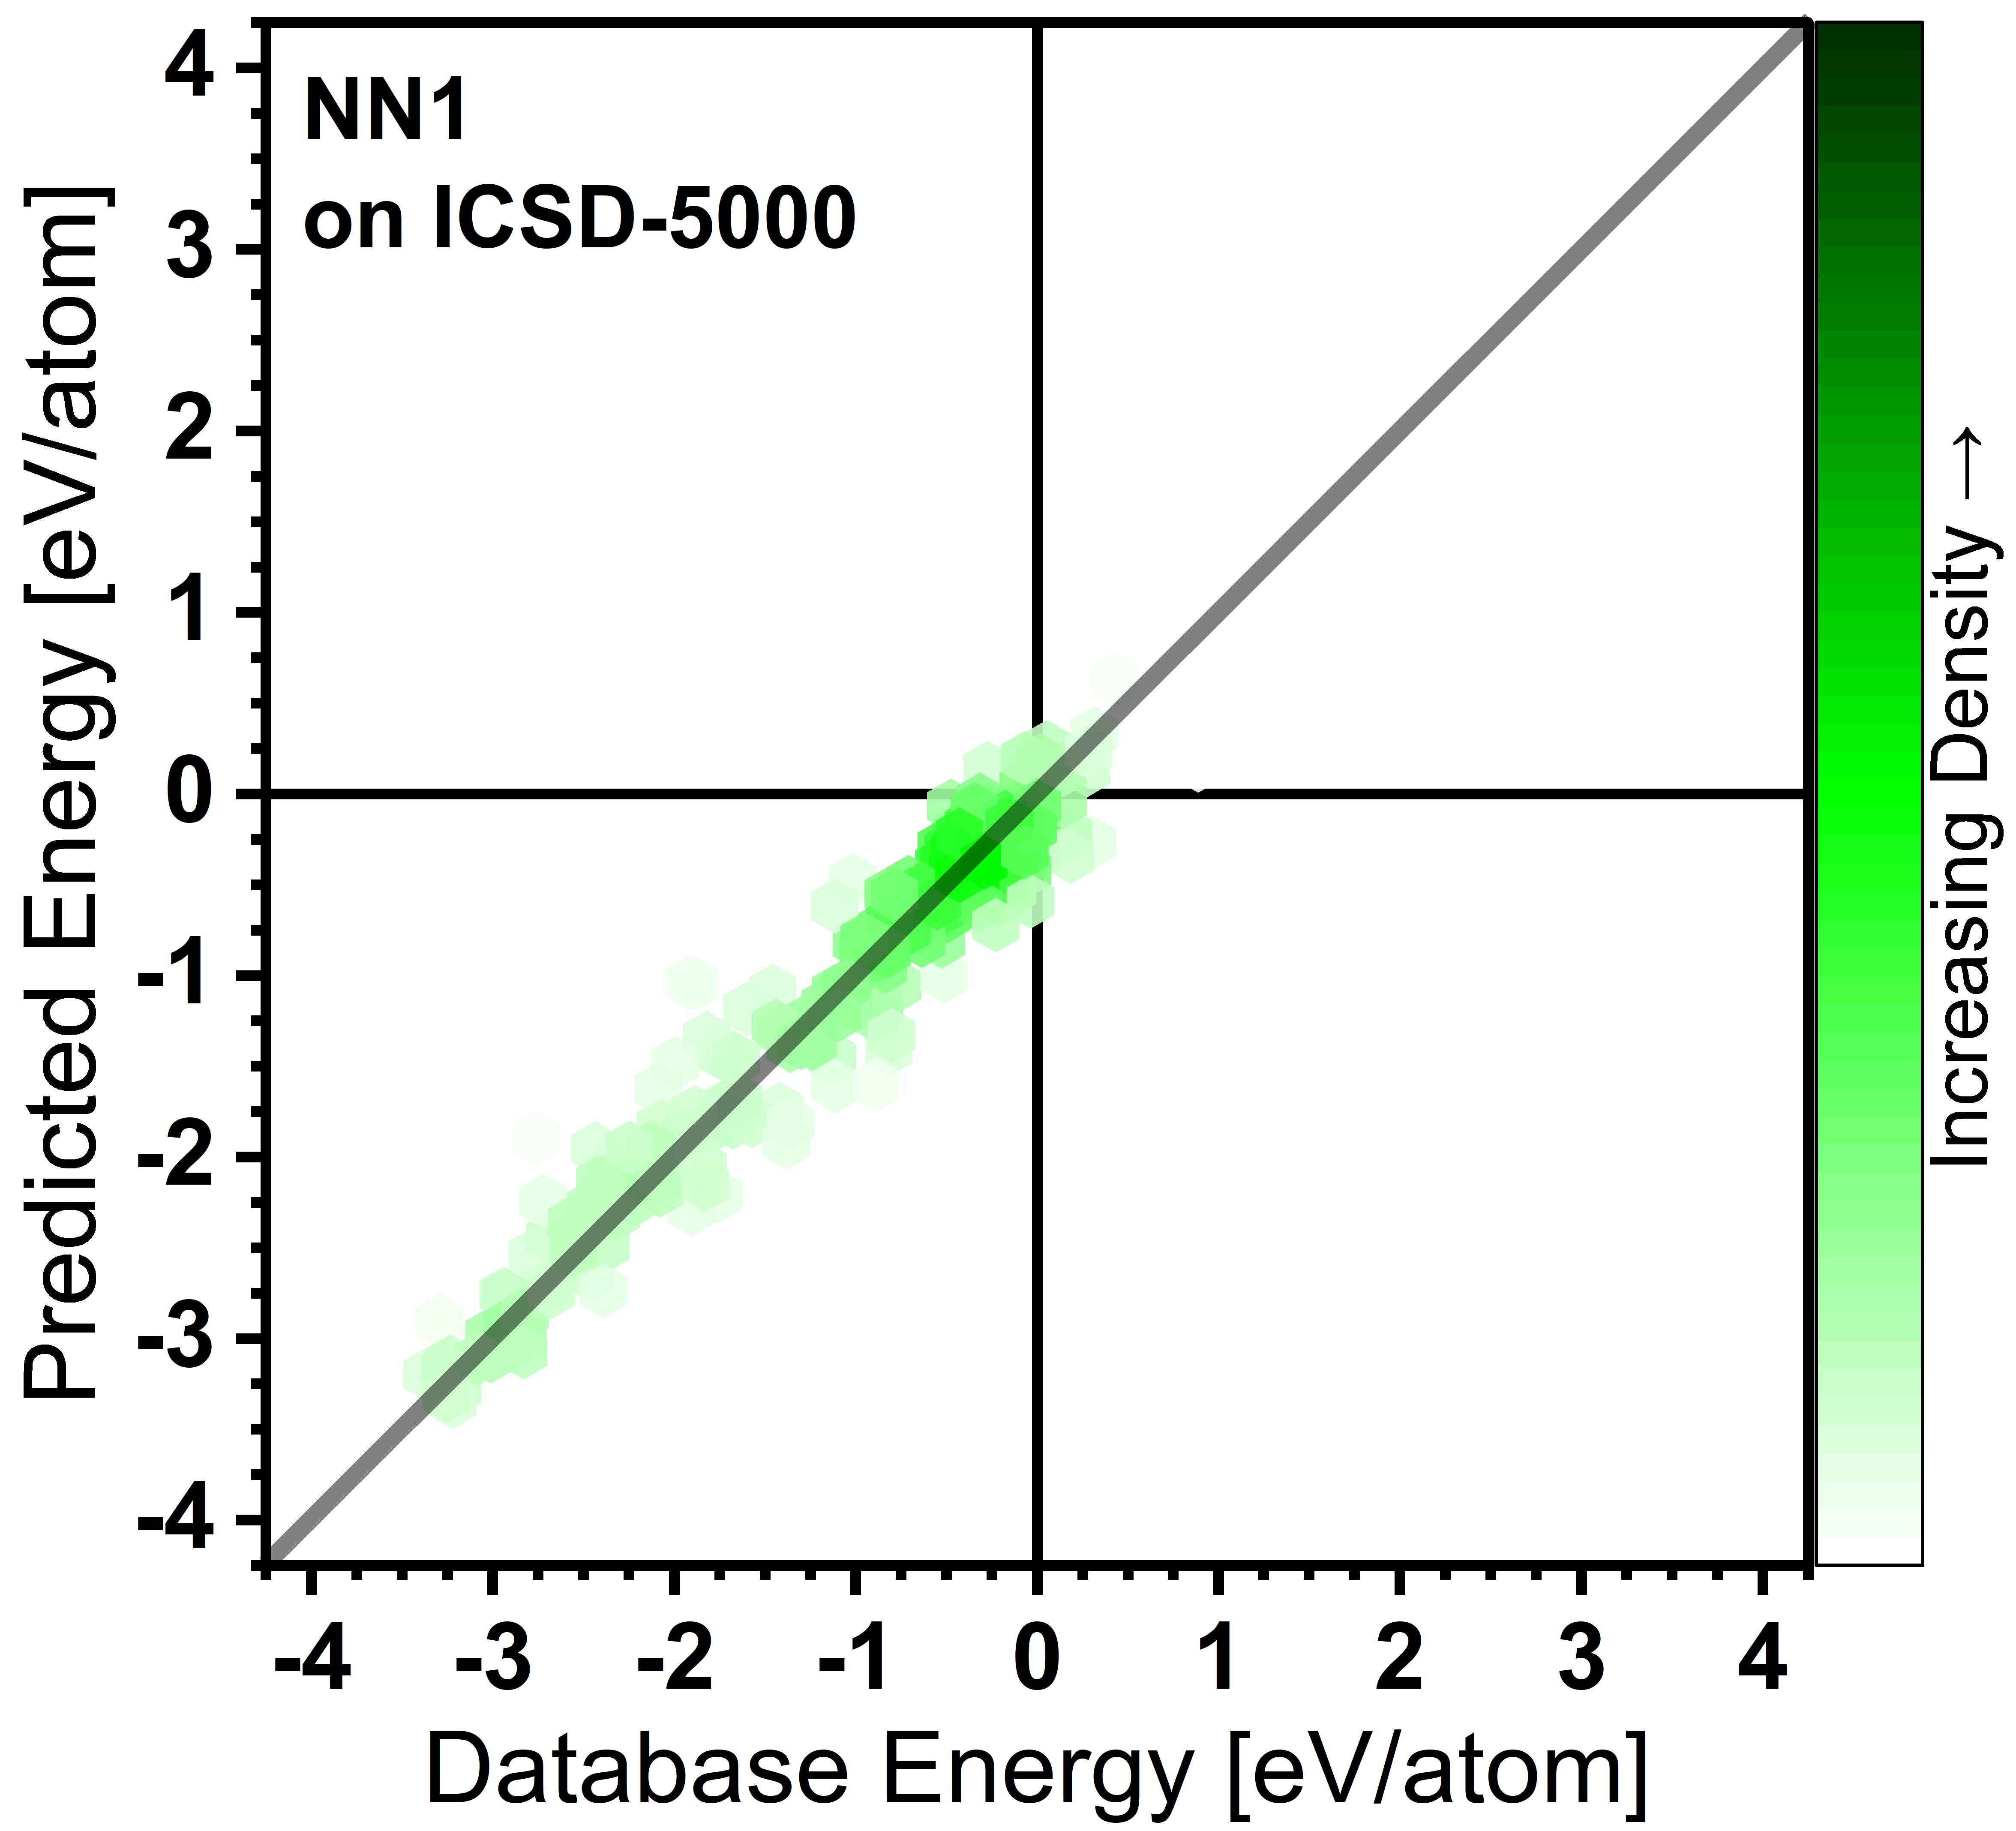
\includegraphics[width=0.35\textwidth]{sipfenn/NN1_test.png}
    \caption{Test of perceptron trained on the data from the first 5000 entries in the ICSD dataset and evaluated on the test set of 230 randomly selected entries ($\approx5\%$)}
    \label{sipfenn:fig:nn1performance}
\end{figure}

When trained on the data from all entries in the ICSD, it achieved an MAE of 364 meV/atom on the test set ($\approx5\% \text{ from } 32116$). This error is comparable to the performance of a random forest model based on PRDF (370 meV/atom), is slightly worse than a CM (250 meV/atom), and is significantly worse than a random-forest model trained on the same descriptor (90 meV/atom), as reported by Ward et al. \cite{Ward2017IncludingTessellations}. Part of the significance of these results is the evident quality of the descriptor, as the model achieved performance that would be considered excellent just a few years prior to the present work while being much less complex and computationally costly. Furthermore, it is important to note the time- and space-complexity of the perceptron model. Training the final network took less than 8 seconds compared to around 10,000 seconds reported for the aforementioned random-forest methods, and the resulting model occupied less than 1kb of memory. Following the testing of a perceptron, which allowed rough estimation of the a good size of the network (i.e. number of weights), the design of the actual architecture began. All of these steps are schematically depicted in Figure \ref{sipfenn:fig:designprocess}.

\begin{figure}[H]
    \centering
    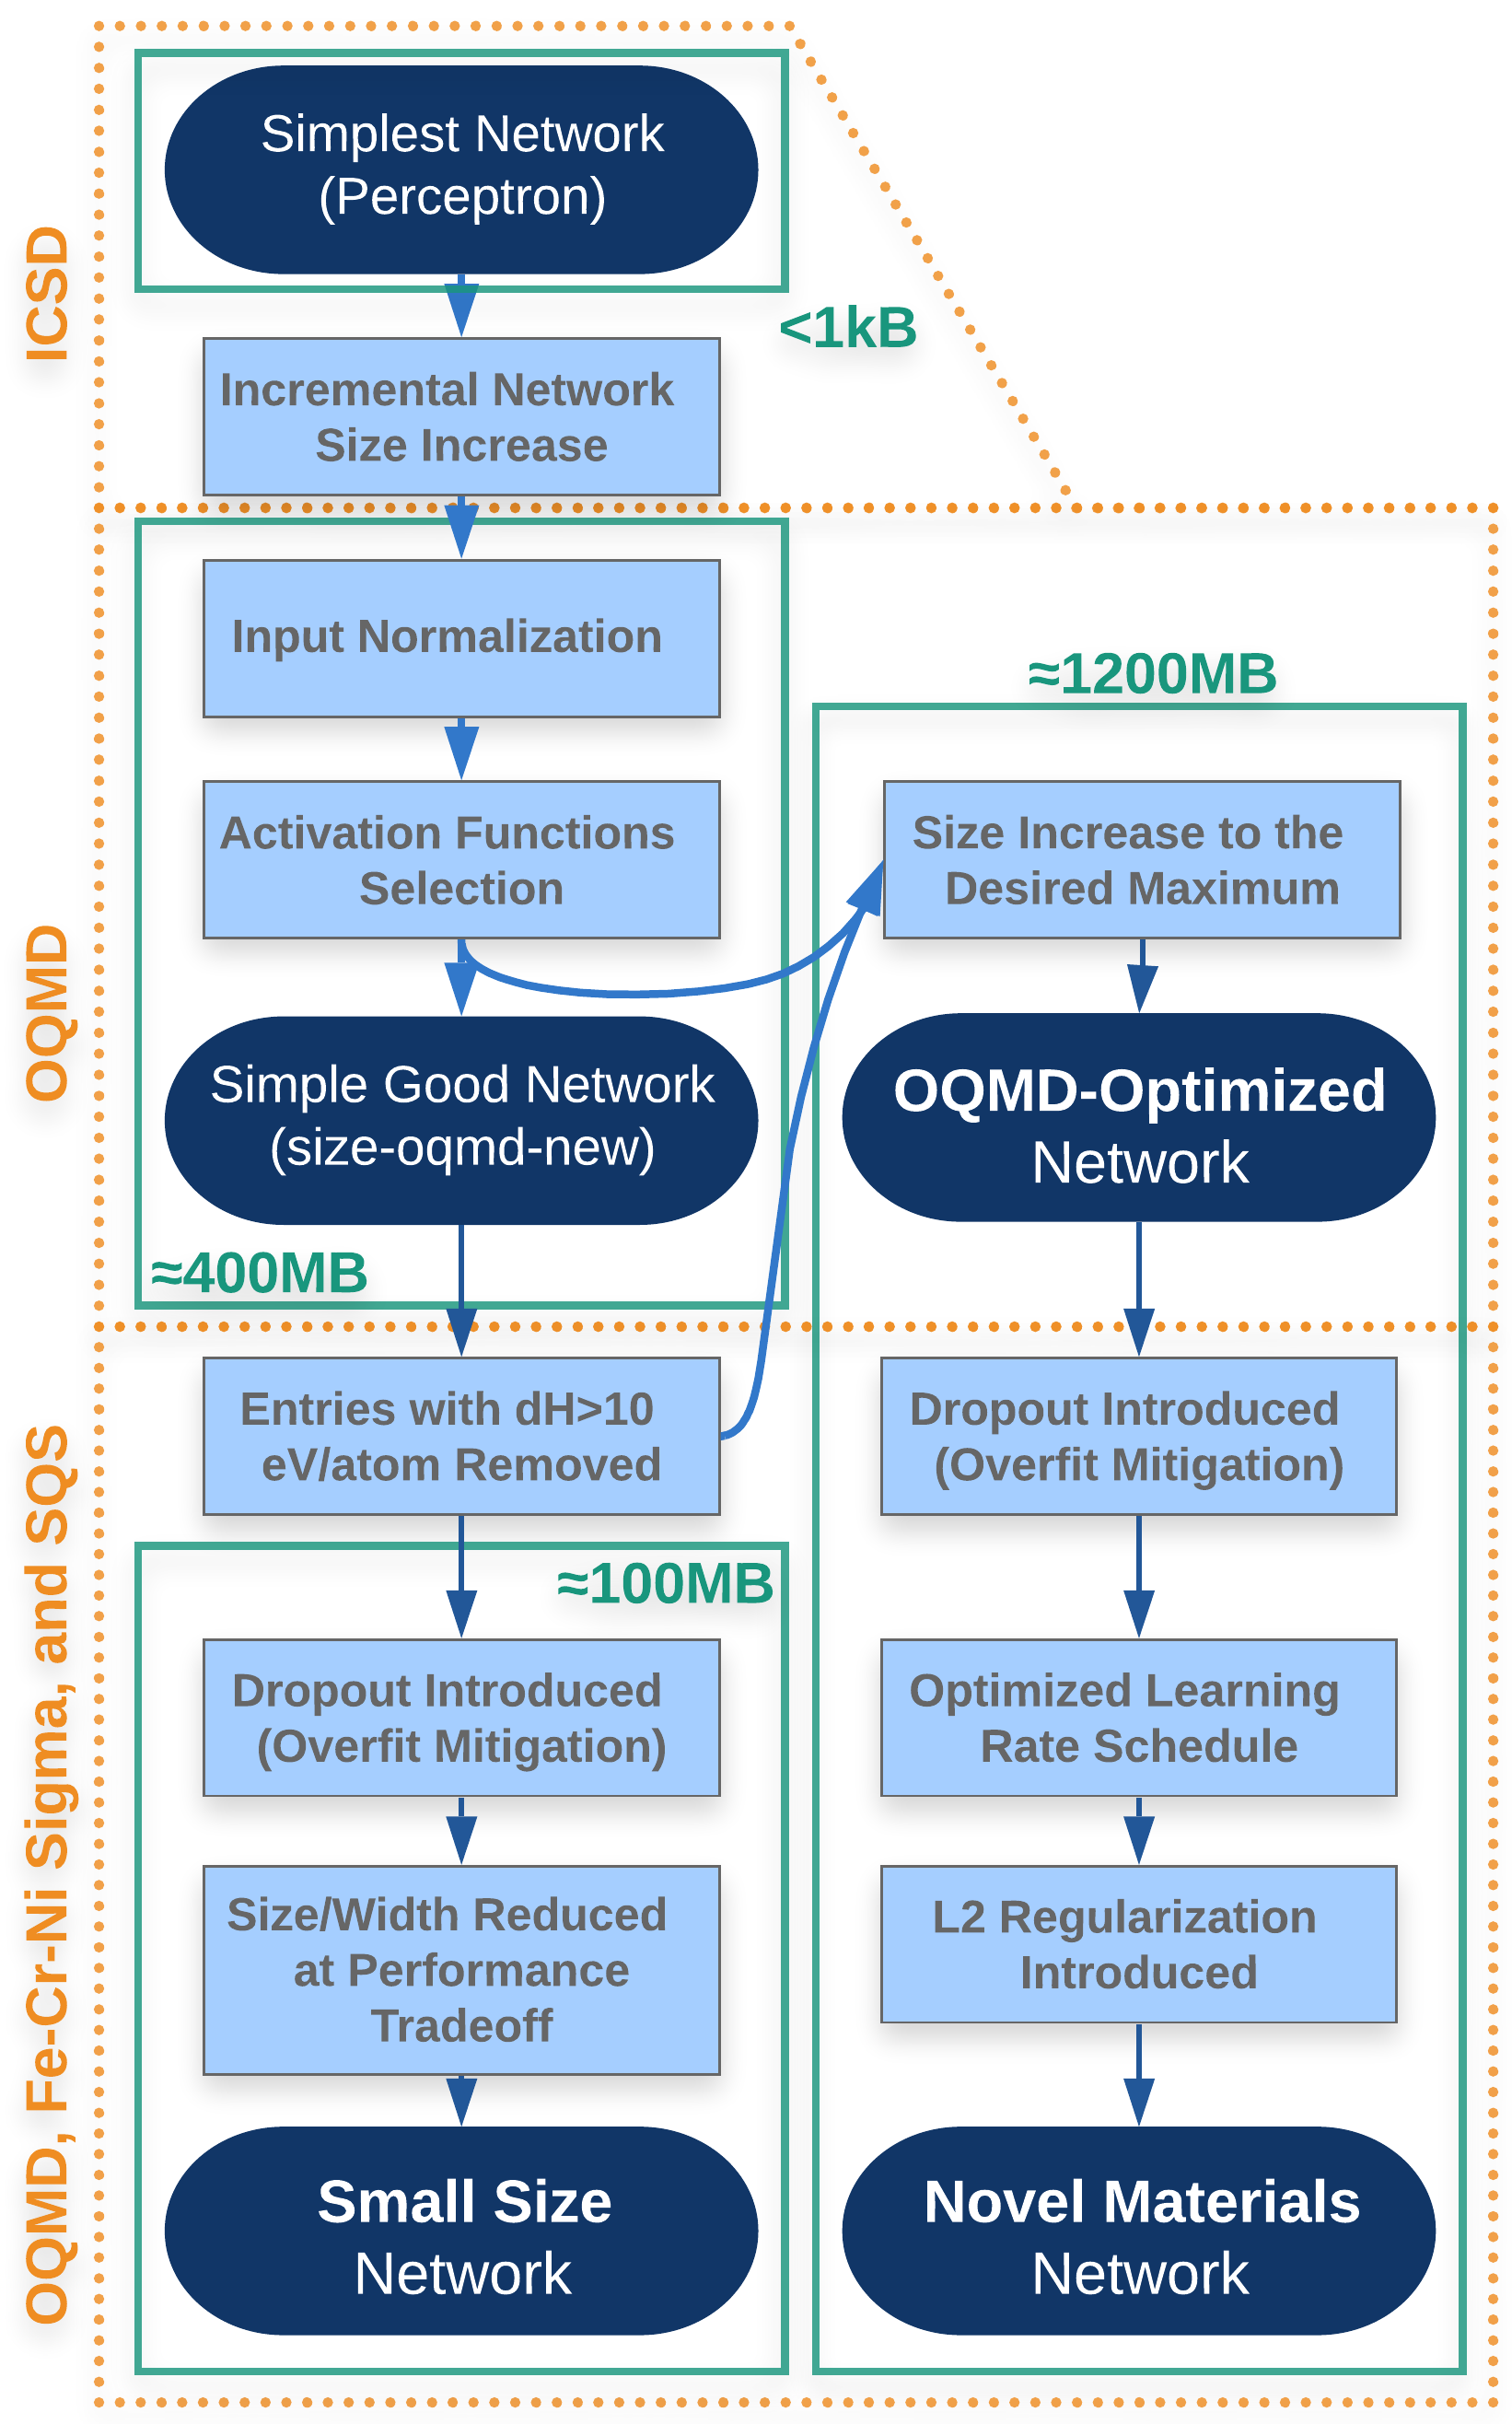
\includegraphics[width=0.5\textwidth]{sipfenn/SIPFENN_design_updated.png}
    \caption{The network design process schematic leading to the three final models. This figure is Figure \ref{sipfenn:fig:designprocess} cloned to the Appendix for conveninece.}
\end{figure}

Next, in a few steps, the size of the network was incrementally increased. First, a layer of 1000 neurons was introduced. This reduced the performance on the first 5000 entries in the ICSD, likely due to overfitting issues, as the data was very limited. Performance on the ICSD was improved, reducing the test MAE to 305 meV/atom on the test set, however. The introduction of the next two 1000-width layers further reduced the MAE to 215 meV/atom. Based on these results, it was estimated that introducing 4 hidden layers with Sigmoid activation function and widths of 10000, 10000, 1000, and 100 would provide good results when trained on the much larger OQMD.

After switching to OQMD, the network exhibited issues with convergence, often predicting a single value for all of the entries. To mitigate this, the descriptor (i.e. network input) was normalized by dividing every element by its maximum value across the whole dataset. This solved the issue. Next, to improve the training behavior, the activation functions were changed from only the Sigmoid function to a mix of Soft Sign, Exponential Linear Unit, and Sigmoid, which was found to work well. These steps improved both the predictive performance and reduced the time required to converge. The network architecture resulting from these steps (internally designated NN8 / Simple Good Network in Figure \ref{sipfenn:fig:designprocess}) was the first to improve performance compared to the Ward et. al approach \cite{Ward2017IncludingTessellations}, achieving an MAE of 42 meV/atom on the test set of random subset 5\% of the OQMD dataset. When testing this network, a small fraction of around 0.03\% of likely incorrect entries in the OQMD was found, as described in \ref{sipfenn:sssec:Data}, and was removed from the dataset used later in the design process.

Once a network with desired performance was obtained, the network size was increased until it either exceeded 1GB or showed signs of extensive overfitting. At the first step of this process, two layers of width 10,000 were added, resulting in a network size of 1.2GB and reduced overfitting, as indicated by the ratio of validation-to-training error lowered from 2.2 to 1.6, relative to NN8. The resulting network (internally designated NN9 / OQMD-Optimized Network in Figure \ref{sipfenn:fig:designprocess}), achieved an MAE of 28 meV/atom on the test set of random subset 5\% of OQMD, which was the best performance on OQMD out of all the networks created in this project. If the 0.03\% of abnormal data wasn't removed as described in \ref{sipfenn:sssec:Data}, it would correspond to, on average, 6 data points which in one tested instance increased the MAE to 35 meV/atom. Important to point out, the training of this network was prone to staying in local minima at the beginning. The reported instance of the trained network exhibited no training progress between around rounds 5 and 25, after which it's performance quickly increased.  Detailed analysis of the performance is given in \ref{sipfenn:ssec:oqmdperformance}.

Once the main objective of the design process was obtained, i.e. the performance on the OQMD has improved appreciably beyond existing methods, the design process was focused on creating a tool for modeling materials that were not reported in the OQMD. Therefore, the objective changed from achieving the lowest MAE on a random subset 5\% of OQMD to (1) reducing the mismatch between training and validation sets errors (i.e. difference between training accuracy and validation accuracy) during the training process, (2) keeping the test MAE on the OQMD below 50 meV/atom, and (3) improving performance on two material groups significantly different from the OQMD data, namely Special Quasirandom Structures (SQS) and Fe-Cr-Ni $\sigma$-phase (see \ref{sipfenn:sssec:Data}).

With these new objectives, two Dropout layers in the middle part of the network were introduced to promote the distribution of pattern recognition abilities across the network. \cite{Srivastava2014Dropout:Overfitting} This introduced a problem with convergence as the network became more likely to fall into local minima at the initial stages of the training, which was solved by introducing custom learning rate schedules. Specifically, the learning rate was initially set to a value orders of magnitude lower than during the default initial training and then ramped up to the previous (ADAM default setting in the majority of frameworks) learning rate of 0.001 (or above) after around 2 rounds of training. This type of learning rate schedule is known as a warm-up in the deep learning literature \cite{gotmare2018closer}. The schedule found to perform the best is presented in Figure \ref{sipfenn:fig:learningrate}.

\begin{figure}[H]
\centering
    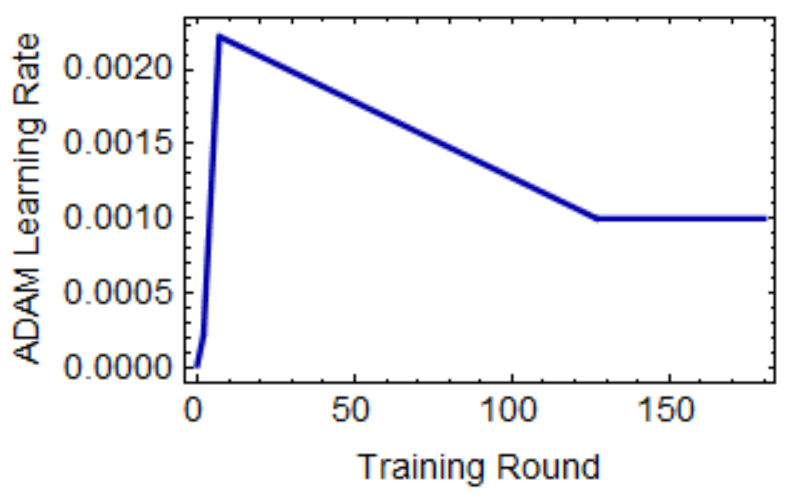
\includegraphics[width=0.35\textwidth]{sipfenn/nn18_learningrate_linonly.png}
    \caption{The learning rate schedule used for training of more complex networks in the later stage of the design process (e.g., NN18).}
    \label{sipfenn:fig:learningrate}
\end{figure}


The next step was the introduction of $\ell^2$ regularization, which is a technique that favors simplification of the descriptor and effectively rejects features of the descriptor that do not contribute to prediction performance \cite{L2Regularization}. An overview on it is given in Section \ref{sipfenn:ref:machinelearningoverview}. In the models reported in the present work an $\ell^2$ value of $10^{-6}$ was used. Higher values were found to stop the training at early stages, impairing the pattern recognition, or in extreme cases (above $10^{-3}$) force the network to discard the input completely, resulting in constant or near-constant output (i.e. mean value from the training dataset predicted for any structure).

The final step was small curation of the training data based on the OQMD-reported structure stability, i.e. the energy difference between the formation energy and the energy convex hull. The motivation for that was the notion that DFT results are inherently less accurate for unstable phases. In this step, all entries with energies of more than 2000 meV/atom above the convex hull were removed from the training set. Importantly, the validation and testing sets were not modified for consistent performance reporting.

All of these changes resulted in a neural network that has been optimized for predicting new materials. In the code and Supplementary materials, it is designated as NN20 (Novel Materials Network in Figure \ref{sipfenn:fig:designprocess}). Compared to the OQMD-optimized network it was derived from, the test MAE on the OQMD increased from 28 to 49 meV/atom. However, at the same time, the mismatch between the training and validation set was reduced from 1.57 to 1.38. Or, as presented earlier in Figure \ref{sipfenn:fig:trainingvalidation}, reduced to about 1.15 for the same training duration. Furthermore, a relatively large portion of this error can be attributed to some unstable structures that were removed from the training set, but not from the test set. Once entries with formation energies of more than 1000 meV/atom above the convex hull were removed, the test MAE decreased to only 38 meV/atom. Restricting the test set further to only somewhat stable structures (stability below 250 meV/atom) resulted in an MAE of 30 meV/atom.

While the new-material-optimized network presented an increased MAE across a random subset of the OQMD, performance has significantly improved on the Fe-Cr-Ni $\sigma-$phase described in \ref{sipfenn:sssec:Data}. The MAE has decreased from 55 to 41 meV/atom, indicating that the model based on this neural network is more capable of making predictions for new materials.

Once two performance-oriented models were developed, increasing the performance-to-cost ratio has been explored with the motivation that some studies would benefit from many times higher throughput at minor accuracy decrease. Architecture design started from the selection of a network with a balanced size-to-performance ratio (NN8) and the introduction of an overfitting mitigation technique (Dropout \cite{srivastava2014dropout}) used for the network optimized for new materials, as depicted in Figure \ref{sipfenn:sssec:NetDesign}. Next, the network was gradually narrowed (fewer neurons in layers) until the performance started to noticeably deteriorate (41.9 meV/atom for 5000- and 4000-width vs 42.1 for 3000-width). This approach allowed a significant reduction of the network size (and the computational intensity to run it) from around 1,200MB of the two other models to around 145MB. If an application demands even more of a reduction in model size and computational cost, the same procedure could be continued until some minimum required performance is retained. 


\section{Feature Ranking Learned During Formation Energy Modeling} 
\label{sipfenn:appendix3}

\begin{longtable}{|l|l|}
\caption{\texttt{SIPFENN}'s \texttt{NN20} Model Input Feature Ranking Learned During Formation Energy Modeling}
\label{sipfenn:appendix3:featureranking}\\
\hline
\multicolumn{1}{|c|}{\textbf{Descriptor Feature}} & \multicolumn{1}{c|}{\textbf{Normalized Squared Weights Sum}} \\ \hline
\endfirsthead
%
\endhead
%
mean\_NeighDiff\_shell1\_MeltingT & 1 \\ \hline
mean\_MeltingT & 0.97502 \\ \hline
max\_MeltingT & 0.73512 \\ \hline
mean\_NeighDiff\_shell1\_NdUnfilled & 0.69157 \\ \hline
MaxPackingEfficiency & 0.68889 \\ \hline
most\_MeltingT & 0.67373 \\ \hline
dev\_GSvolume\_pa & 0.61042 \\ \hline
var\_NeighDiff\_shell1\_Column & 0.58782 \\ \hline
var\_NeighDiff\_shell1\_CovalentRadius & 0.57826 \\ \hline
var\_NeighDiff\_shell1\_MeltingT & 0.57259 \\ \hline
maxdiff\_GSvolume\_pa & 0.55156 \\ \hline
dev\_MeltingT & 0.5286 \\ \hline
mean\_SpaceGroupNumber & 0.51761 \\ \hline
min\_MeltingT & 0.50437 \\ \hline
var\_CellVolume & 0.49467 \\ \hline
var\_NeighDiff\_shell1\_MendeleevNumber & 0.492 \\ \hline
min\_NeighDiff\_shell1\_MeltingT & 0.47853 \\ \hline
mean\_NeighDiff\_shell1\_Column & 0.45566 \\ \hline
maxdiff\_CovalentRadius & 0.42998 \\ \hline
var\_NeighDiff\_shell1\_Electronegativity & 0.42642 \\ \hline
var\_EffectiveCoordination & 0.40506 \\ \hline
min\_NeighDiff\_shell1\_Column & 0.39822 \\ \hline
dev\_NdUnfilled & 0.39739 \\ \hline
dev\_CovalentRadius & 0.36935 \\ \hline
range\_NeighDiff\_shell1\_Column & 0.35956 \\ \hline
range\_NeighDiff\_shell1\_CovalentRadius & 0.34585 \\ \hline
mean\_WCMagnitude\_Shell1 & 0.34275 \\ \hline
mean\_NeighDiff\_shell1\_MendeleevNumber & 0.33911 \\ \hline
mean\_EffectiveCoordination & 0.33899 \\ \hline
mean\_Number & 0.33769 \\ \hline
mean\_NdUnfilled & 0.33408 \\ \hline
maxdiff\_MeltingT & 0.33348 \\ \hline
mean\_AtomicWeight & 0.33149 \\ \hline
mean\_NeighDiff\_shell1\_NdValence & 0.33142 \\ \hline
range\_NeighDiff\_shell1\_MeltingT & 0.33107 \\ \hline
max\_NfUnfilled & 0.33041 \\ \hline
dev\_Electronegativity & 0.33001 \\ \hline
mean\_NeighDiff\_shell1\_CovalentRadius & 0.32999 \\ \hline
var\_NeighDiff\_shell1\_NdUnfilled & 0.31973 \\ \hline
dev\_Column & 0.31662 \\ \hline
var\_NeighDiff\_shell1\_NdValence & 0.31481 \\ \hline
mean\_WCMagnitude\_Shell2 & 0.31359 \\ \hline
most\_NfUnfilled & 0.30916 \\ \hline
MeanIonicChar & 0.30732 \\ \hline
mean\_NeighDiff\_shell1\_Electronegativity & 0.30277 \\ \hline
min\_EffectiveCoordination & 0.29705 \\ \hline
min\_NeighDiff\_shell1\_CovalentRadius & 0.29392 \\ \hline
max\_NeighDiff\_shell1\_GSvolume\_pa & 0.2875 \\ \hline
most\_SpaceGroupNumber & 0.28472 \\ \hline
max\_NdUnfilled & 0.28424 \\ \hline
maxdiff\_NdUnfilled & 0.28405 \\ \hline
var\_NeighDiff\_shell1\_GSvolume\_pa & 0.28008 \\ \hline
min\_BondLengthVariation & 0.27922 \\ \hline
var\_MeanBondLength & 0.2768 \\ \hline
dev\_NdValence & 0.27566 \\ \hline
max\_NeighDiff\_shell1\_MeltingT & 0.27097 \\ \hline
max\_BondLengthVariation & 0.26565 \\ \hline
mean\_NfValence & 0.26558 \\ \hline
mean\_NsUnfilled & 0.2612 \\ \hline
max\_NeighDiff\_shell1\_CovalentRadius & 0.26026 \\ \hline
max\_GSvolume\_pa & 0.25985 \\ \hline
min\_GSvolume\_pa & 0.25895 \\ \hline
mean\_NdValence & 0.25573 \\ \hline
mean\_NeighDiff\_shell1\_GSvolume\_pa & 0.25299 \\ \hline
max\_NValance & 0.24749 \\ \hline
range\_NeighDiff\_shell1\_NdUnfilled & 0.24643 \\ \hline
max\_CovalentRadius & 0.23136 \\ \hline
CanFormIonic & 0.23135 \\ \hline
min\_NeighDiff\_shell1\_Electronegativity & 0.22873 \\ \hline
min\_SpaceGroupNumber & 0.22766 \\ \hline
max\_Electronegativity & 0.22609 \\ \hline
max\_NdValence & 0.22576 \\ \hline
most\_NdUnfilled & 0.22198 \\ \hline
min\_NeighDiff\_shell1\_MendeleevNumber & 0.21991 \\ \hline
var\_NeighDiff\_shell1\_NpValence & 0.21609 \\ \hline
min\_NeighDiff\_shell1\_NdUnfilled & 0.2114 \\ \hline
dev\_SpaceGroupNumber & 0.2099 \\ \hline
most\_NfValence & 0.20888 \\ \hline
min\_MeanBondLength & 0.2086 \\ \hline
mean\_BondLengthVariation & 0.20507 \\ \hline
var\_NeighDiff\_shell1\_Row & 0.20454 \\ \hline
max\_NeighDiff\_shell1\_NdUnfilled & 0.20318 \\ \hline
min\_NeighDiff\_shell1\_NdValence & 0.20123 \\ \hline
min\_CovalentRadius & 0.19974 \\ \hline
range\_NeighDiff\_shell1\_MendeleevNumber & 0.19591 \\ \hline
min\_NeighDiff\_shell1\_GSvolume\_pa & 0.19565 \\ \hline
most\_NpUnfilled & 0.19457 \\ \hline
maxdiff\_NUnfilled & 0.19316 \\ \hline
max\_NeighDiff\_shell1\_NdValence & 0.19307 \\ \hline
max\_NpValence & 0.1929 \\ \hline
range\_NeighDiff\_shell1\_GSvolume\_pa & 0.19166 \\ \hline
most\_NdValence & 0.1904 \\ \hline
max\_MeanBondLength & 0.19021 \\ \hline
maxdiff\_NfUnfilled & 0.18897 \\ \hline
max\_NeighDiff\_shell1\_Column & 0.18518 \\ \hline
range\_NeighDiff\_shell1\_Electronegativity & 0.18322 \\ \hline
var\_NeighDiff\_shell1\_SpaceGroupNumber & 0.18313 \\ \hline
dev\_NpValence & 0.18099 \\ \hline
mean\_NpUnfilled & 0.18091 \\ \hline
range\_NeighDiff\_shell1\_SpaceGroupNumber & 0.17858 \\ \hline
dev\_MendeleevNumber & 0.17753 \\ \hline
MaxIonicChar & 0.176 \\ \hline
mean\_Column & 0.17206 \\ \hline
min\_Electronegativity & 0.17164 \\ \hline
mean\_WCMagnitude\_Shell3 & 0.17077 \\ \hline
mean\_Row & 0.17035 \\ \hline
min\_NeighDiff\_shell1\_SpaceGroupNumber & 0.17031 \\ \hline
most\_NsUnfilled & 0.16714 \\ \hline
var\_BondLengthVariation & 0.16653 \\ \hline
var\_NeighDiff\_shell1\_NfUnfilled & 0.16223 \\ \hline
range\_NeighDiff\_shell1\_NdValence & 0.16094 \\ \hline
frac\_fValence & 0.1609 \\ \hline
maxdiff\_Column & 0.16083 \\ \hline
max\_NUnfilled & 0.15916 \\ \hline
mean\_NpValence & 0.15639 \\ \hline
maxdiff\_NpValence & 0.15637 \\ \hline
mean\_MendeleevNumber & 0.15491 \\ \hline
most\_Electronegativity & 0.15469 \\ \hline
mean\_Electronegativity & 0.15458 \\ \hline
max\_SpaceGroupNumber & 0.15429 \\ \hline
dev\_Row & 0.15382 \\ \hline
maxdiff\_MendeleevNumber & 0.15373 \\ \hline
var\_NeighDiff\_shell1\_NpUnfilled & 0.15135 \\ \hline
max\_NeighDiff\_shell1\_Electronegativity & 0.15115 \\ \hline
most\_NUnfilled & 0.14955 \\ \hline
max\_GSbandgap & 0.14945 \\ \hline
mean\_NeighDiff\_shell1\_NUnfilled & 0.14891 \\ \hline
maxdiff\_NValance & 0.14819 \\ \hline
mean\_NeighDiff\_shell1\_NpValence & 0.14768 \\ \hline
maxdiff\_NdValence & 0.14735 \\ \hline
max\_NpUnfilled & 0.14647 \\ \hline
maxdiff\_Electronegativity & 0.14523 \\ \hline
min\_MendeleevNumber & 0.14119 \\ \hline
mean\_CovalentRadius & 0.14049 \\ \hline
mean\_NeighDiff\_shell1\_Row & 0.13945 \\ \hline
maxdiff\_GSbandgap & 0.13891 \\ \hline
max\_NeighDiff\_shell1\_MendeleevNumber & 0.13858 \\ \hline
most\_Number & 0.13823 \\ \hline
most\_AtomicWeight & 0.13798 \\ \hline
max\_NeighDiff\_shell1\_NpValence & 0.13757 \\ \hline
Comp\_L10Norm & 0.13598 \\ \hline
min\_Row & 0.13596 \\ \hline
range\_NeighDiff\_shell1\_NpValence & 0.13524 \\ \hline
mean\_GSvolume\_pa & 0.1331 \\ \hline
max\_NeighDiff\_shell1\_NUnfilled & 0.13205 \\ \hline
mean\_NeighDiff\_shell1\_NfValence & 0.12888 \\ \hline
min\_NeighDiff\_shell1\_NpUnfilled & 0.12778 \\ \hline
mean\_NeighDiff\_shell1\_SpaceGroupNumber & 0.12722 \\ \hline
mean\_NsValence & 0.12642 \\ \hline
most\_CovalentRadius & 0.12616 \\ \hline
var\_NeighDiff\_shell1\_NUnfilled & 0.12525 \\ \hline
mean\_NeighDiff\_shell1\_Number & 0.12466 \\ \hline
Comp\_L7Norm & 0.12293 \\ \hline
mean\_NeighDiff\_shell1\_AtomicWeight & 0.12229 \\ \hline
min\_NeighDiff\_shell1\_NpValence & 0.12026 \\ \hline
max\_EffectiveCoordination & 0.11995 \\ \hline
min\_NdValence & 0.11984 \\ \hline
maxdiff\_NpUnfilled & 0.11976 \\ \hline
mean\_NeighDiff\_shell1\_NsUnfilled & 0.11836 \\ \hline
max\_NeighDiff\_shell1\_GSbandgap & 0.11657 \\ \hline
min\_NUnfilled & 0.11648 \\ \hline
most\_Column & 0.1164 \\ \hline
var\_NeighDiff\_shell1\_Number & 0.11483 \\ \hline
most\_MendeleevNumber & 0.11312 \\ \hline
max\_NeighDiff\_shell1\_SpaceGroupNumber & 0.11292 \\ \hline
var\_NeighDiff\_shell1\_AtomicWeight & 0.11234 \\ \hline
most\_NpValence & 0.11231 \\ \hline
frac\_dValence & 0.11126 \\ \hline
NComp & 0.11097 \\ \hline
min\_Number & 0.11062 \\ \hline
range\_NeighDiff\_shell1\_NpUnfilled & 0.11002 \\ \hline
dev\_NValance & 0.10868 \\ \hline
min\_Column & 0.10846 \\ \hline
max\_NeighDiff\_shell1\_NpUnfilled & 0.10837 \\ \hline
maxdiff\_Row & 0.10735 \\ \hline
Comp\_L5Norm & 0.10726 \\ \hline
mean\_NeighDiff\_shell1\_NpUnfilled & 0.10682 \\ \hline
maxdiff\_SpaceGroupNumber & 0.10604 \\ \hline
dev\_GSbandgap & 0.10604 \\ \hline
max\_AtomicWeight & 0.10495 \\ \hline
max\_GSmagmom & 0.10416 \\ \hline
maxdiff\_GSmagmom & 0.1039 \\ \hline
dev\_NUnfilled & 0.10336 \\ \hline
var\_NeighDiff\_shell1\_NfValence & 0.10059 \\ \hline
dev\_GSmagmom & 0.10046 \\ \hline
most\_GSbandgap & 0.09997 \\ \hline
var\_NeighDiff\_shell1\_NValance & 0.09842 \\ \hline
min\_NeighDiff\_shell1\_Row & 0.09798 \\ \hline
min\_NeighDiff\_shell1\_NUnfilled & 0.09563 \\ \hline
most\_Row & 0.09538 \\ \hline
max\_Number & 0.0925 \\ \hline
most\_GSvolume\_pa & 0.09166 \\ \hline
mean\_GSbandgap & 0.09097 \\ \hline
range\_NeighDiff\_shell1\_Row & 0.09081 \\ \hline
mean\_NValance & 0.0889 \\ \hline
mean\_NeighDiff\_shell1\_NsValence & 0.08449 \\ \hline
min\_NsValence & 0.08408 \\ \hline
frac\_pValence & 0.08403 \\ \hline
mean\_NUnfilled & 0.08244 \\ \hline
mean\_NfUnfilled & 0.08194 \\ \hline
dev\_NpUnfilled & 0.0818 \\ \hline
dev\_Number & 0.08065 \\ \hline
max\_NeighDiff\_shell1\_GSmagmom & 0.08049 \\ \hline
max\_Column & 0.07989 \\ \hline
min\_AtomicWeight & 0.07959 \\ \hline
Comp\_L3Norm & 0.07913 \\ \hline
max\_NeighDiff\_shell1\_Row & 0.0776 \\ \hline
mean\_NeighDiff\_shell1\_NValance & 0.07619 \\ \hline
mean\_NeighDiff\_shell1\_NfUnfilled & 0.07413 \\ \hline
range\_NeighDiff\_shell1\_NfUnfilled & 0.07381 \\ \hline
min\_NValance & 0.07297 \\ \hline
max\_NeighDiff\_shell1\_NValance & 0.0726 \\ \hline
range\_NeighDiff\_shell1\_NfValence & 0.07163 \\ \hline
min\_NdUnfilled & 0.07145 \\ \hline
most\_NsValence & 0.07114 \\ \hline
mean\_NeighDiff\_shell1\_GSbandgap & 0.06709 \\ \hline
max\_NfValence & 0.06661 \\ \hline
dev\_AtomicWeight & 0.06581 \\ \hline
maxdiff\_Number & 0.06576 \\ \hline
max\_NeighDiff\_shell1\_NfUnfilled & 0.06523 \\ \hline
dev\_NfUnfilled & 0.06477 \\ \hline
dev\_NfValence & 0.06373 \\ \hline
range\_NeighDiff\_shell1\_GSmagmom & 0.06305 \\ \hline
var\_NeighDiff\_shell1\_NsUnfilled & 0.06288 \\ \hline
min\_NeighDiff\_shell1\_Number & 0.0623 \\ \hline
frac\_sValence & 0.06099 \\ \hline
min\_NeighDiff\_shell1\_NfValence & 0.06033 \\ \hline
max\_Row & 0.05998 \\ \hline
min\_NeighDiff\_shell1\_NValance & 0.05844 \\ \hline
range\_NeighDiff\_shell1\_NUnfilled & 0.05819 \\ \hline
var\_NeighDiff\_shell1\_GSbandgap & 0.05683 \\ \hline
range\_NeighDiff\_shell1\_AtomicWeight & 0.0568 \\ \hline
Comp\_L2Norm & 0.05638 \\ \hline
min\_NeighDiff\_shell1\_NsUnfilled & 0.05541 \\ \hline
most\_NValance & 0.0553 \\ \hline
maxdiff\_NsValence & 0.05459 \\ \hline
range\_NeighDiff\_shell1\_NValance & 0.0537 \\ \hline
min\_NeighDiff\_shell1\_AtomicWeight & 0.05369 \\ \hline
max\_NsValence & 0.05329 \\ \hline
range\_NeighDiff\_shell1\_GSbandgap & 0.05299 \\ \hline
min\_NeighDiff\_shell1\_NfUnfilled & 0.05266 \\ \hline
maxdiff\_NfValence & 0.05147 \\ \hline
dev\_NsUnfilled & 0.04884 \\ \hline
max\_MendeleevNumber & 0.04844 \\ \hline
maxdiff\_AtomicWeight & 0.04814 \\ \hline
max\_NeighDiff\_shell1\_NsUnfilled & 0.04675 \\ \hline
max\_NeighDiff\_shell1\_NsValence & 0.04663 \\ \hline
var\_NeighDiff\_shell1\_GSmagmom & 0.04635 \\ \hline
range\_NeighDiff\_shell1\_Number & 0.04416 \\ \hline
max\_NeighDiff\_shell1\_NfValence & 0.04376 \\ \hline
mean\_NeighDiff\_shell1\_GSmagmom & 0.0433 \\ \hline
most\_GSmagmom & 0.04239 \\ \hline
range\_NeighDiff\_shell1\_NsUnfilled & 0.03954 \\ \hline
min\_NeighDiff\_shell1\_NsValence & 0.03932 \\ \hline
max\_NeighDiff\_shell1\_AtomicWeight & 0.03905 \\ \hline
max\_NeighDiff\_shell1\_Number & 0.03815 \\ \hline
min\_NfValence & 0.03794 \\ \hline
dev\_NsValence & 0.0373 \\ \hline
maxdiff\_NsUnfilled & 0.03558 \\ \hline
min\_NfUnfilled & 0.03537 \\ \hline
min\_NeighDiff\_shell1\_GSmagmom & 0.03353 \\ \hline
var\_NeighDiff\_shell1\_NsValence & 0.02948 \\ \hline
min\_NpValence & 0.02946 \\ \hline
max\_NsUnfilled & 0.02933 \\ \hline
min\_NeighDiff\_shell1\_GSbandgap & 0.02735 \\ \hline
mean\_GSmagmom & 0.02402 \\ \hline
min\_NpUnfilled & 0.02233 \\ \hline
range\_NeighDiff\_shell1\_NsValence & 0.02171 \\ \hline
min\_NsUnfilled & 0.02051 \\ \hline
min\_GSbandgap & 0.01299 \\ \hline
min\_GSmagmom & 0.00132 \\ \hline
\end{longtable}

\section{Extended Statistics and Visualizations of Materials-Property-Descriptor Database} \label{mpdd:app1}

The three key statistics presented in Figure~\ref{mpdd:fig:dataset} are a small subset of the larger dashboard available at \href{https://phaseslab.org/mpdd}{phaseslab.org/mpdd} web page, which is presented in Figure~\ref{sup:mpdd:dashboard}.

\begin{figure}[H]
    \centering
    
\includegraphics[width=0.95\textwidth]{mpdd/mpdddashboard.png}
    \caption{The main MPDD dashboard with statistics over MPDD dataset, as of April 2024, demonstrating the dataset in terms of different levels of "corese-graining" the uniqueness criteria, and coverage of chemical systems of different order.}
    \label{sup:mpdd:dashboard}
\end{figure}

Partial data on all of the MPDD data points can be accessed through a graphical user interface (GUI), available at \href{https://mpdd.org}{mpdd.org}, presented in Figure~\ref{sup:mpdd:gui}. It enables users to query the database based on fields including chemical formula, chemical system, or space group number, to facilitate easy access for users not familiar with programming and those who only need to access a small subset of it.

\begin{figure}[H]
    \centering
    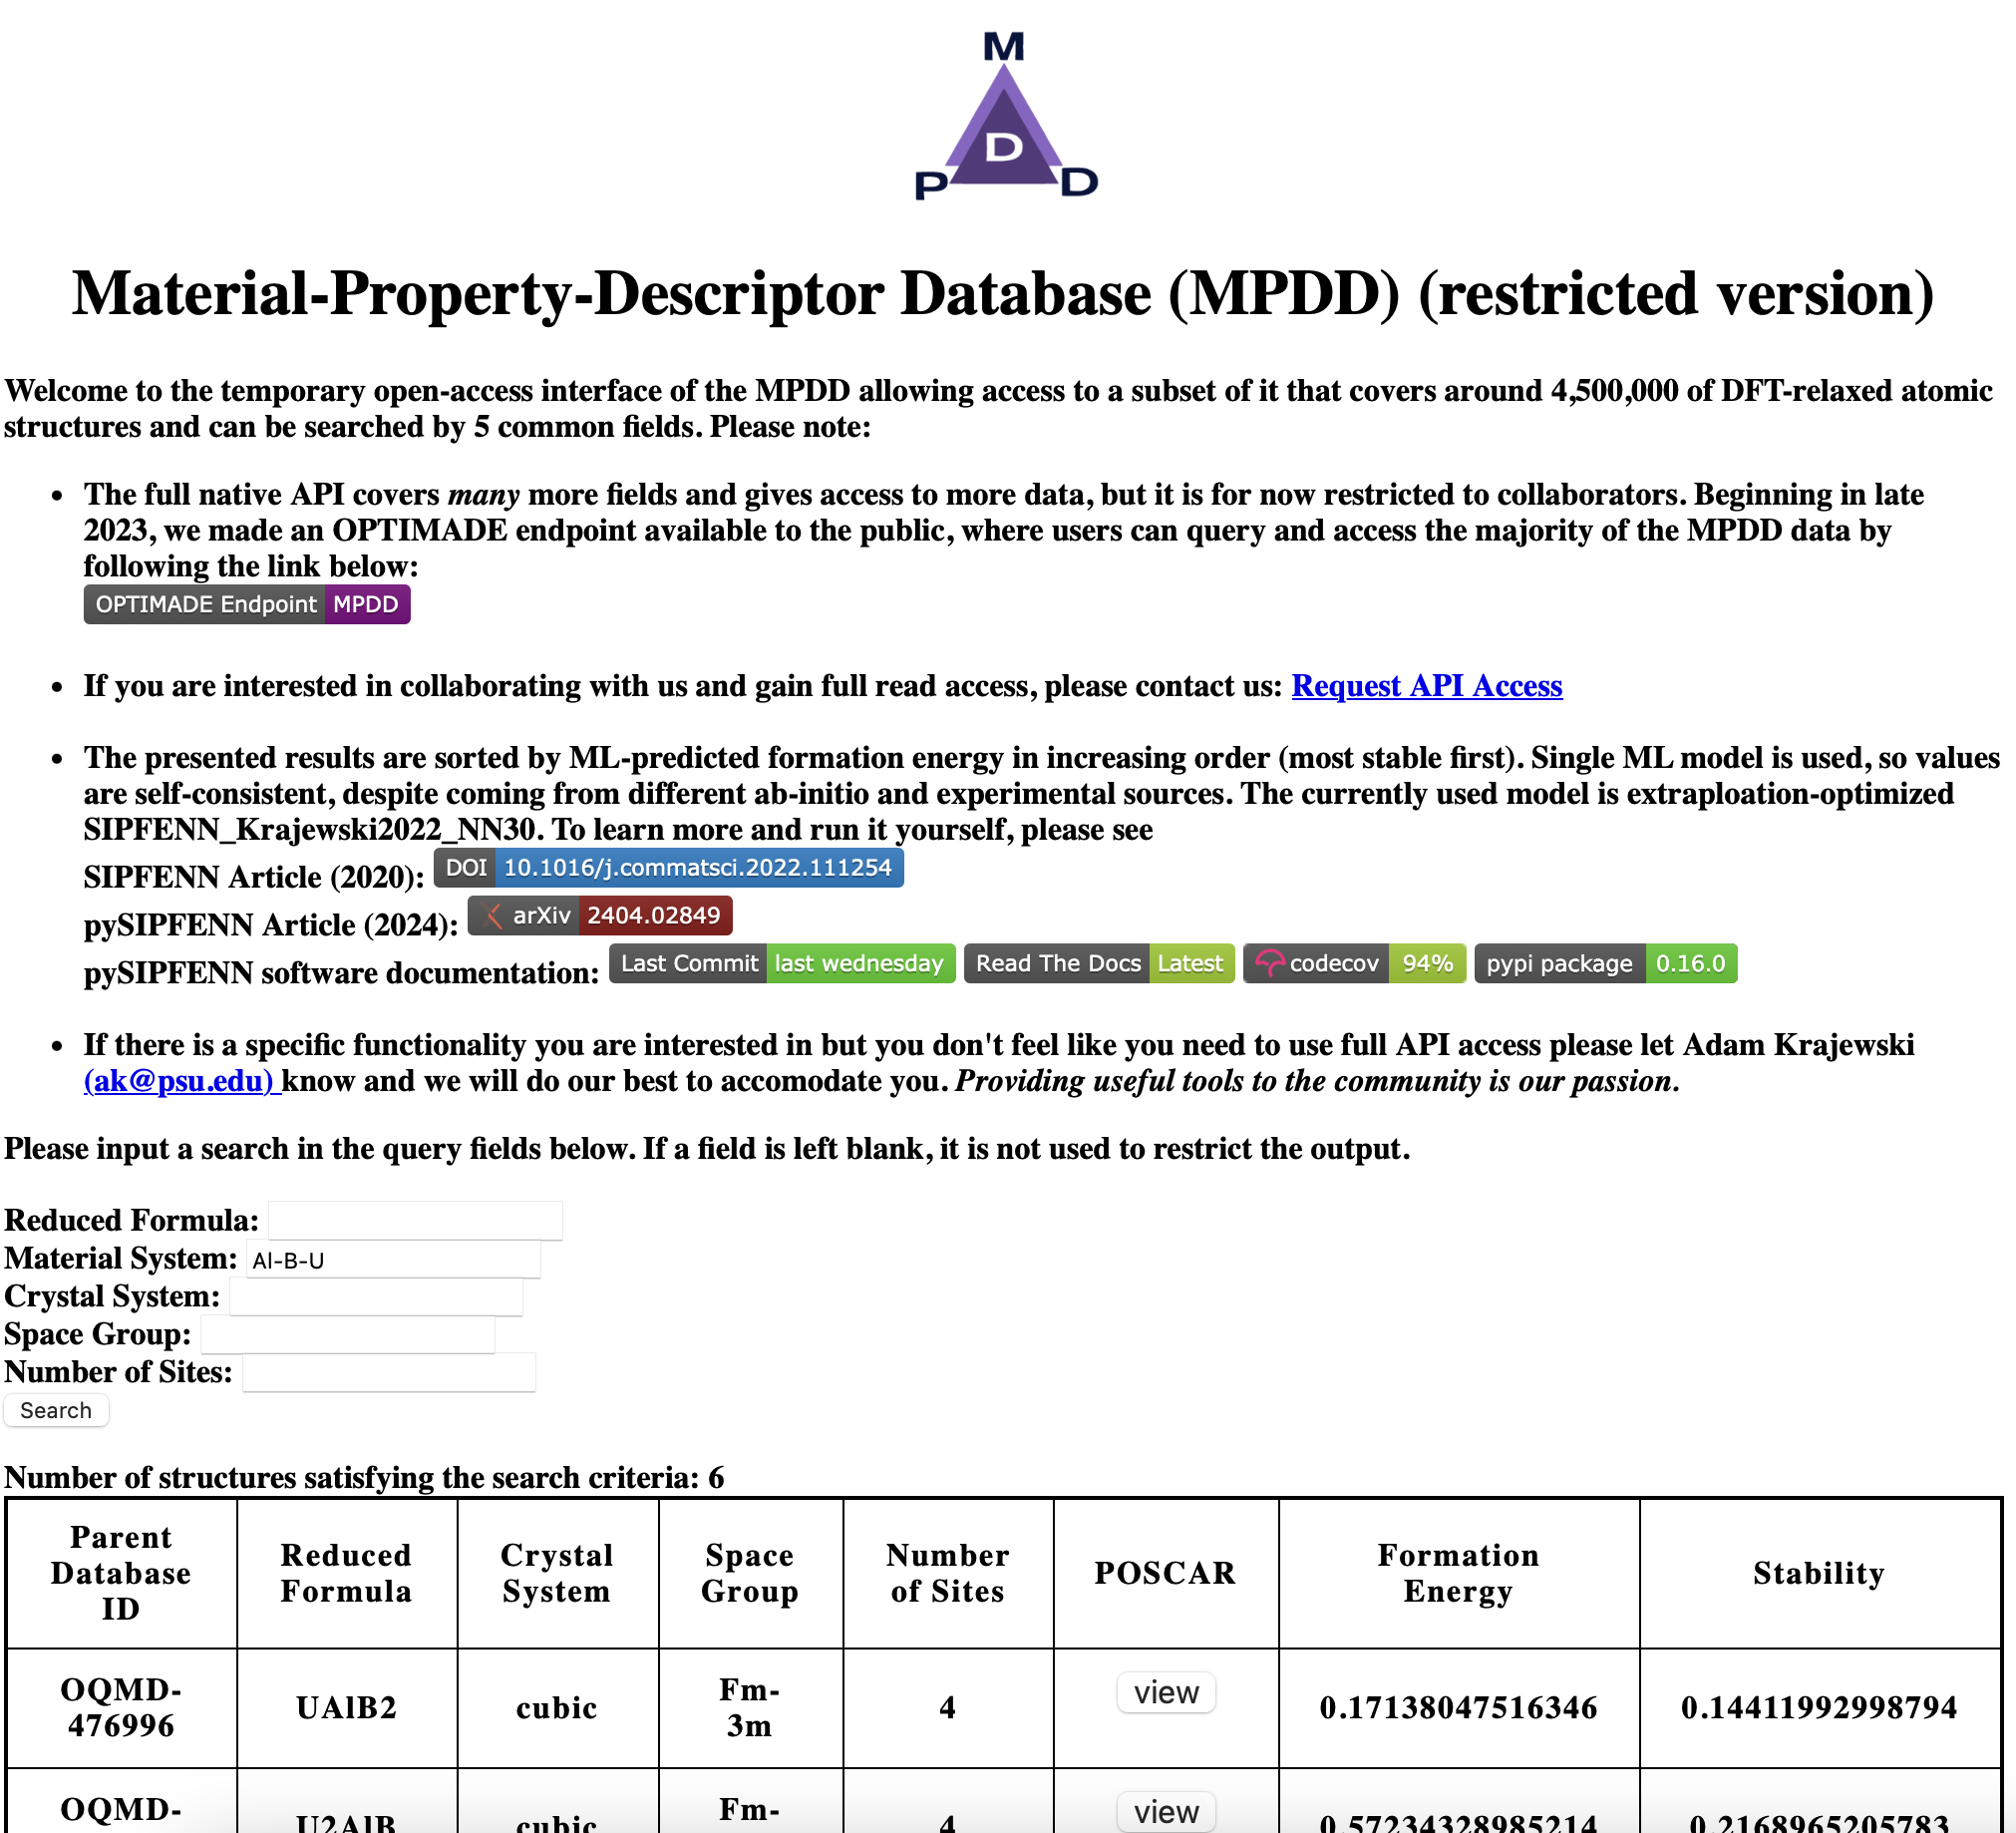
\includegraphics[width=0.95\textwidth]{mpdd/mpddgui.png}
    \caption{A basic MPDD graphical user interface (GUI) set up for easy access to the data based on a couple of common query fields.}
    \label{sup:mpdd:gui}
\end{figure}

The OPTIMADE API \cite{Evans2024DevelopmentsExchange}, as discussed in Section~\ref{mpdd:sec:optimade}, can be accessed using software like \texttt{optimade-python-tools} \cite{Evans2021} or by going to the \href{http://optimade.mpdd.org}{optimade.mpdd.org} endpoint. Figure~\ref{sup:mpdd:optimade} depicts the expected web page, as of May 2024.

\begin{figure}[H]
    \centering
    
\includegraphics[width=0.9\textwidth]{mpdd/mpddoptimade.png}
    \caption{Printout of the MPDD OPTIMADE API endpoint page.}
    \label{sup:mpdd:optimade}
\end{figure}

One can use the endpoint page shown in Figure~\ref{sup:mpdd:optimade} to quickly check (1) accessibility of the database, and (2) investigate its schema, by following endpoint like \href{http://optimade.mpdd.org/v1/structures}{optimade.mpdd.org/v1/structures} to see example data response, like the one shown in Figure~\ref{sup:mpdd:optimadeout}, or \href{http://optimade.mpdd.org/v1/info}{optimade.mpdd.org/v1/info} to see MPDD provider information page.

\begin{figure}[H]
    \centering
    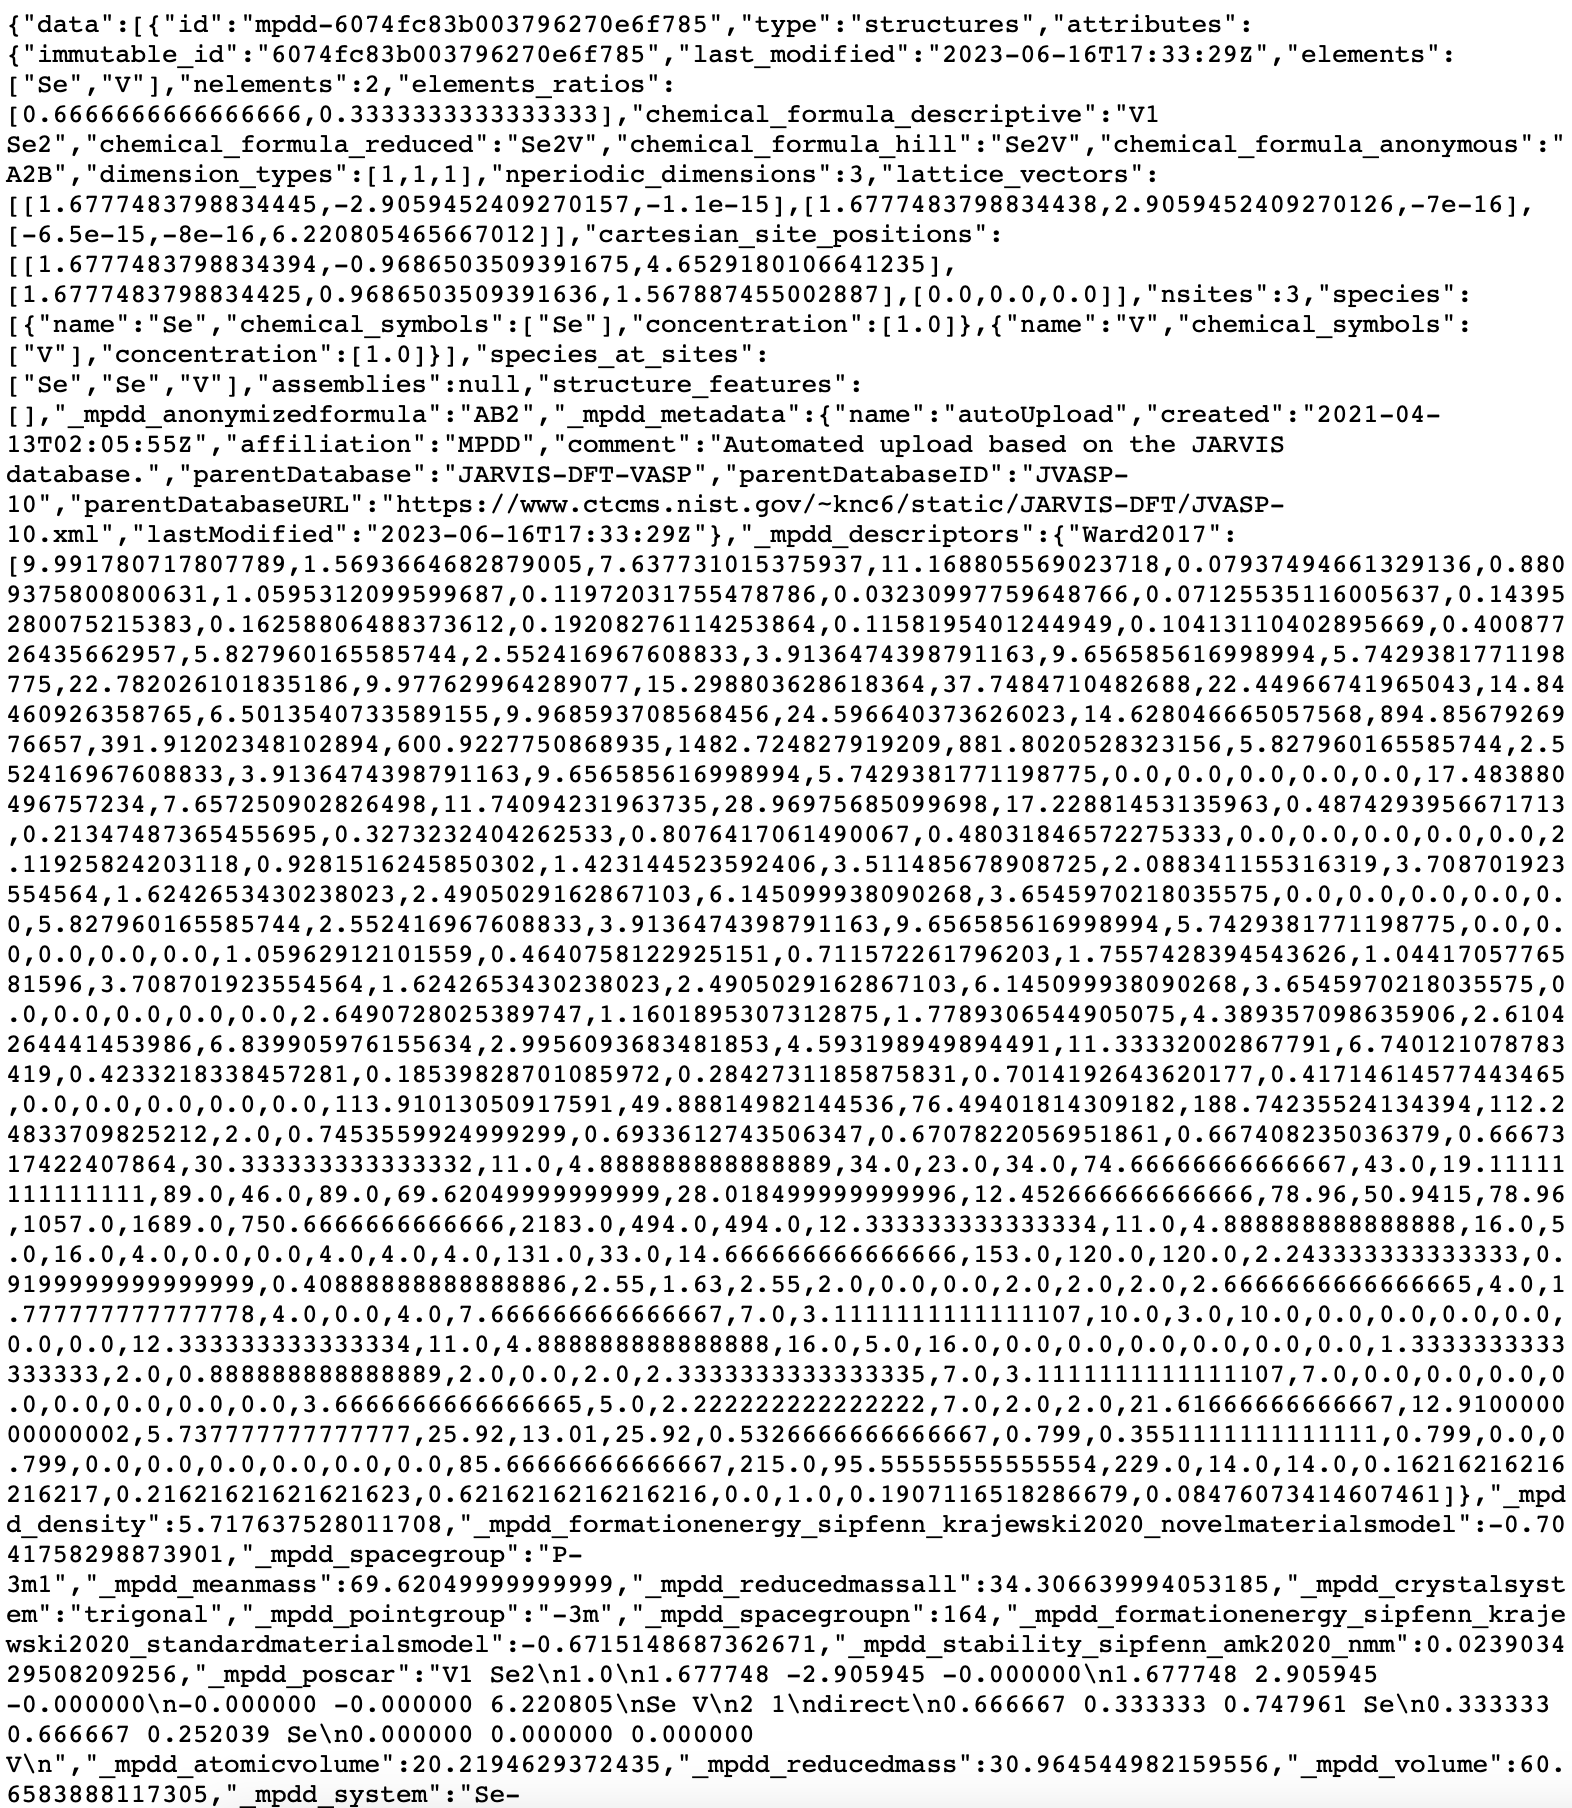
\includegraphics[width=0.95\textwidth]{mpdd/mpddoptimadeout.png}
    \caption{An example printout of (partial) MPDD's OPTIMADE response upon a query to the \texttt{http://optimade.mpdd.org/v1/structures} endpoint, depicting human-unreadable but machine-readable output.}
    \label{sup:mpdd:optimadeout}
\end{figure}


\section{Motivation for Multi-Grade Compositional Design of Materials Exemplified with Hf-Zr Powders} \label{nimplex:app1}

As mentioned in Section~\ref{nimplex:ssec:functionallygraded}, different grades of base metals may have very different costs associated with them. For instance, as of December 2023, at \href{https://www.fishersci.com}{Fisher Scientific online store (fishersci.com)}, one can purchase:
\begin{itemize}
    \item High-purity Zr wire: $250cm$ of $0.25mm$-diameter (AA00416CB) for $\$317$ or $\approx 390\frac{\$}{g}$
    \item $99.2\%$ (Zr+$4.5\%$Hf) wire: $200cm$ of $0.25mm$-diameter (AA43334G2) for $\$63$ or $\approx 100\frac{\$}{g}$. 
    \item $99.97\%$ (Hf+$3\%$Zr) wire: $200cm$ of $0.25mm$-diameter (AA10200G2) for $\$200$ or $\approx 156\frac{\$}{g}$. 
\end{itemize} 

Now, if one tries to create FGMs which navigates Zr-rich regions in Hf-containing space, there are two possible choices for Zr source, namely, pure Zr or the (Zr+$4.5\%Hf$) alloy. The first one enables all possible Zr fractions, unlike the latter which establishes the minimum Hf fraction at 4.5\% at the "Zr" corner of the attainable space tetrahedron (anonymous example of this is in Figure~\ref{nimplex:fig:fgmspaces}). Such an ability may be necessary, e.g., to avoid infeasible regions of space, but if not, it represents an unnecessary cost. 

For instance, to obtain (Zr+$10\%wt$Hf) alloy, one can combine high-purity Zr and (Hf+$3\%Zr$) for $\approx 360\frac{\$}{g}$ or equivalently from (Zr+$4.5\%$Hf) and (Hf+$3\%$Zr) for $\approx 103\frac{\$}{g}$, representing 3.5 times cost reduction.

At Fisher Scientific, as of writing this, the pure-Zr wire is only available in $0.25mm$ diameter, thus, the above considerations were restricted to it to keep the comparisons fair. However, for the (Zr+$4.5\%$Hf) grade, many less-expensive form factors are available as it is much more industry relevant. Furthermore, larger package sizes ($\geq50g$) are available driving the cost down further. For instance, the following $1mm$ wires can be purchased:

\begin{itemize}
    \item $99.2\%$ (Zr+$4.5\%$Hf) wire: $10m$ of $1mm$-diameter  (AA14627H2) for $\$130$ or $\approx 2.5\frac{\$}{g}$. 
    \item $99.97\%$ (Hf+$3\%$Zr) wire: $5m$ of $1mm$-diameter (AA10205CC) for $\$580$ or $\approx 11.3\frac{\$}{g}$. 
\end{itemize}

If the above are used, one can now obtain the same (Zr+$10\%wt$Hf) alloy for $\approx 3\frac{\$}{g}$ or 120 times cheaper relative to using high purity Zr in the only available physical form factor.
    

\section{Geometric Cross-Evidence for Factorial Decay of Simplex Space in Equally Dimensional Cartesian Space}  \label{nimplex:app2}

The equation for the fraction of a cube bound by [111] plane, equivalent to the result for $f(4)$ in Section~\ref{nimplex:sec:randomuniformsampling}, can be quickly obtained by considering that the volume of a pyramid is given by $V = \frac{A_B h}{3}$, where $A_B$ is the base area of equilateral triangle $\frac{\sqrt{3}}{4}\times\sqrt{2}^2 = \frac{\sqrt{3}}{2}$ and $h$ is $\frac{1}{\sqrt{3}}$. Thus we get 
$$V = \frac{\frac{\sqrt{3}}{2} \frac{1}{\sqrt{3}}}{3} = \frac{1}{6}$$ 
agreeing with the aforementioned result in Section~\ref{nimplex:sec:randomuniformsampling}.


\section{Bidirectional \texttt{neighborsLink4C} Algorithm found Conceptually}  \label{nimplex:app3}

The equation for "forward" and "backward" jumps in 3-simplex graph corresponding to a quaternary chemical system. 

\begin{minted}[xleftmargin=3\parindent, fontsize=\small]{nim}
proc neighborsLink4C(
    i:int, x:Tensor, neighbors: var seq[seq[int]], ndiv: int): void =
  let jump0 = 1  #binom(x, 0)=1
  let jump1 = binom(1+ndiv-x[0]-x[1], 1)
  let jump2 = binom(2+ndiv-x[0], 2)
  
  if x[0] != 0:
    # quaternary
    neighbors[i].add(i - jump2)
    # quaternary
    neighbors[i].add(i - jump2 - jump1)
    # quaternary
    neighbors[i].add(i - jump2 - jump1 - jump0) 
  
  if x[1] != 0:
    # ternary
    neighbors[i].add(i - jump1)    
    # ternary
    neighbors[i].add(i - jump1 - jump0)         
    # quaternary
    neighbors[i].add(i + jump2 - jump1 - x[1])  
  
  if x[2] != 0:
    # binary
    neighbors[i].add(i - jump0)     
    # ternary
    neighbors[i].add(i + jump1 - jump0)    
    # quaternary
    neighbors[i].add(i + jump2 - jump0 - x[1])  
  
  if x[3] != 0:
    # binary
    neighbors[i].add(i + jump0)        
    # ternary
    neighbors[i].add(i + jump1)          
    # quaternary     
    neighbors[i].add(i + jump2 - x[1])              
\end{minted}

%\printbibliography[heading=subbibintoc]